
\section{Flüsse und Schnitte}

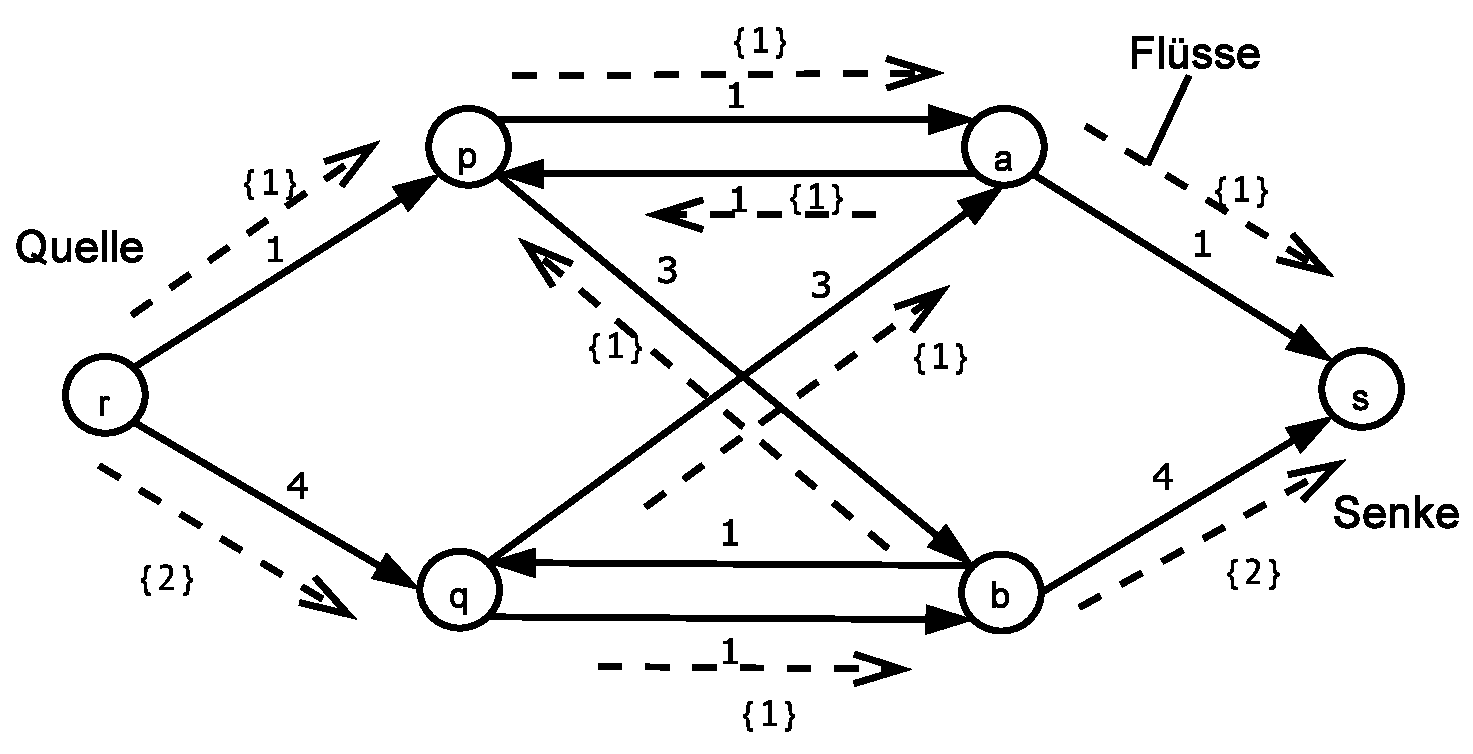
\includegraphics[height=4cm]{bilder/3-0Maxfluss}

Die Flüsse können nun als Kollektion von einfachen $(r,s)$-Wegen (die nicht
notwendigerweise verschieden sind) betrachtet werden. In der Grafik sind
allerdings nur die kumulierten Flüsse dargestellt. $\{ p_{1}, p_{2}, \ldots
p_{k} \}$ mit:
\begin{enumerate}
\item jedes $e \in E$ ist höchstens $u_{e}$
\item die Anzahl der Wege werden maximiert
\[ x_{e} = | \{ i | P_{i} \mbox{ benutzt } e\} |\]
\end{enumerate}
Bedingungen für $x$:\\
\[ (\ast) \hspace{3mm} \sum_{w \in V, \; w v \in E} x_{w v} - \sum_{w\in V,
\; v w \in E} x_{v w} = 0\]
\[(\ast \ast) \hspace{3mm} 0 \leqq x_{v w} \leqq u_{v w} \forall \; v w \in E\]
$x_{v w}$ ist ganzzahlig $\forall v w \in E$. Die Zielfunktion lautet:
\[ max \sum_{w \in V,\;  w s \in E} x_{w s} - \sum _{w \in V,\;   s w \in E}
x_{s w} = k \mbox{ ( $=$ Flusswert})\]

Damit haben wir das Maximum ganzzahlige Flussproblem formuliert.

$x \in R^{E}$ heißt Fluss, falls $x$ $(\ast)$ erfüllt.\\
$x \in R^{E}$ heißt zulässiger Fluss, falls $x$ $(\ast \ast)$ erfüllt.

$f_{x} (v) := \displaystyle \sum_{w \in V, \; w v \in E} x_{w v} -  \sum_{w \in V, \; v w
\in E} x_{v  w}$ Dies nennt man auch "`Nettofluss"' oder "`Überschuss"' bei
$v$

$(\ast)  = f_{x}(v) = 0 $ ist die "`Flusserhaltungsbedingung"' und $f_{s}$
ist der Flusswert.

\begin{lemma} \label{Familie}
Eine Familie $\{P_{1}, P_{2},\ldots, P_{k}\}$ von $(r,s)$-Wegen mit $|\{i |
P_{i} \mbox{ benutzt }e\}| \leqq u_{e}$ existiert genau dann wenn ein
ganzzahliger zulässiger $(r,s)$-Fluss mit Flusswert $k$ existiert.
\end{lemma}

Beweis: $\exists$ Familie von Wegen $\Rightarrow \exists$ ein Fluss,
klar.\\
"`$\Leftarrow$"' Gegeben sein ein Fluss $x \in R^{e}$ mit Flusswert $k$.
Entferne Kreise:
\[ x_{e} := x_{e} -1 \; \; \forall \; e \in \mbox{ Kreis } C\]
$\Rightarrow$ Flusswert $k$ bleibt.

Finde $P_{1}$ : $v \ldots s$ (mit alle n Kanten $> 0$) $x_{e} := x_{e} -1
\forall \; e \in P_{1}$. $\rightarrow$ Flusswert ist $k-1$.

Finde $P_{k}$

\paragraph{Maximales Flussproblem} \mbox{}\\
\[\begin{array}{rcl}
\max f_{x}(s)\\
f_{x}(v) &=&0 \; \; \forall v \in V \wout \{r,s\}\\
0 \leqq x_{e} &\leqq& u_{e} \; \; \forall\; e \in E
\end{array}\]

Für einen Kreisfluss der Menge $\alpha$ gilt: $0 < \alpha \leqq \min
\{u_{e}, e \in C\}$

\begin{lemma}
Jeder zulässige $(r,s)$-Fluss ist die Summe von höchstens $m$ Kreis und
Weg-Flüssen.
\end{lemma}

Beweis: Analog zu \ref{Familie} mit Kreis und Wegeflüssen.

\subsubsection{Maximale Flüsse und minimale Schnitte}

Definition des gerichteten Schnittes $R$:
\[ R \subseteq V, \; \; \delta(R) = \{v w | v w \in E, \; v \in R, \; w \not\in
R\}\]
Ein $(r,s)$-gerichteter Schnitt: $r \in R, \; s \not\in R$\\
$A \subseteq V, \; \bar{A} := V \wout A \hspace{3mm} \delta(v)$ für
$\delta(\{v\})$, $\delta(\bar{v})$ für $\delta(\bar{\{v\}})$.

\begin{lemma}\label{SchnittFluss}
Für jeden $(r,s)$-Schnitt $\delta(R)$ und jeden $(r,s)$-Fluss $x$ gilt
$x(\delta(R))$ - $x(\delta(\bar{R})) = f_{x}(s)$
\end{lemma}

Im Beispiel: $R=\{r,q,p\} \Rightarrow 4-1 = 3$

Beweis: 
\[\begin{array}{rcl}
\displaystyle \sum_{v \in \bar{R} \wout \{s\}} f_{x}(v) &=&0\\
f_{x} (s) &=& f_{x}(s)\\
\mbox{addiert: } \hspace{3mm} \displaystyle \sum_{v \in \bar{R}} f_{x}(v)
&=& f_{x}(s) 
\end{array}\]

Wenn Kante $e$ beide Endpunkte in $R$ hat:
\[\begin{array}{rcl}
e = v w, \; v,w \in R&:& \mbox{tritt nicht auf, 0-Koeffizient in Summe}\\
v, w \in \bar{R}&:& \begin{array}[t]{l}
\left. \begin{array}{l} 
\mbox{$v$-Gleichung, Koeffizient -1}\\
\mbox{$w$-Gleichung, Koeffizient 1}
\end{array}
\right\} \mbox{Koeffizient 0} \end{array}\\
v \in R, \; w \not\in  R&:& \mbox{Koeffizient 1}\\
v \not\in R, \; w \in R&:& \mbox{Koeffizient -1}
\end{array}
\]
$f_{x}(v) = \displaystyle \sum_{w v \in E} x_{w v} - \sum_{v w \in E}
x_{v w}$\\
$\Rightarrow \displaystyle \sum_{v \in R} f_{x}(v) = x(\delta(R)) - x (\delta(\bar{R}))
\hspace{3mm} \mbox{q.e.d.}$

\begin{korollar}\label{FlussSchnittKap}
Für jeden zulässigen $(r,s)$-Fluss $x$ und jeden $(r,s)$-Schnitt
$\delta(R)$ gilt:
\[f_{x}(s) \leqq u (\delta(R)) \hspace{7mm} \mbox{$u = $ Kapazität}\]
\end{korollar}
Im Beispiel: $ R = \{r,p,q\} \rightarrow f_{x}(s)\leqq 8$

Beweis: $\begin{array}[t]{rcl}
x(\delta(R)) &\leqq & u (\delta(R))\\
-x (\delta(\bar{R})) &\leqq &0\\
\stackrel{\ref{SchnittFluss}}{\Rightarrow} f_{x}(s) &\leqq & u (\delta(R))
\hspace{3mm} \mbox{q.e.d.}
\end{array}$\\
Dies ist ähnlich zur schwachen Dualität.


\begin{satz}\label{MaxFlowMinCut}
Max Flow Min Cut Theorem\\
Gibt es einen maximalen $(r,s)$-Fluss, so gilt
\[\max\{f_{x}(s) | x \mbox{ ist zul. $(r,s)$-Fluss}\} = 
\min \{u(\delta(R))| \delta (R) \mbox{ ist ein $(r,s)$-Schnitt}\}\]
\end{satz}
(entspricht der starken Dualität)

Beweisidee:
\begin{enumerate}
\item Finde $(r,s)$-Weg $P$ mit $x_{e} < u_{e} \forall \; e \in P$
\item Erhöhe Fluss (alle $x_{e} \in P$) um $\min\{u_{e} - x_{e} | e \in
P\}$
\end{enumerate}
Im Beispiel: kein maximaler Fluss, trotzdem funktioniert diese Idee nicht.

Generalisierung: $\forall$ Vorwärtskanten $x_{e} < u_{e}$ und $\forall$
Rückwärtskanten $x_{e} > 0$ 

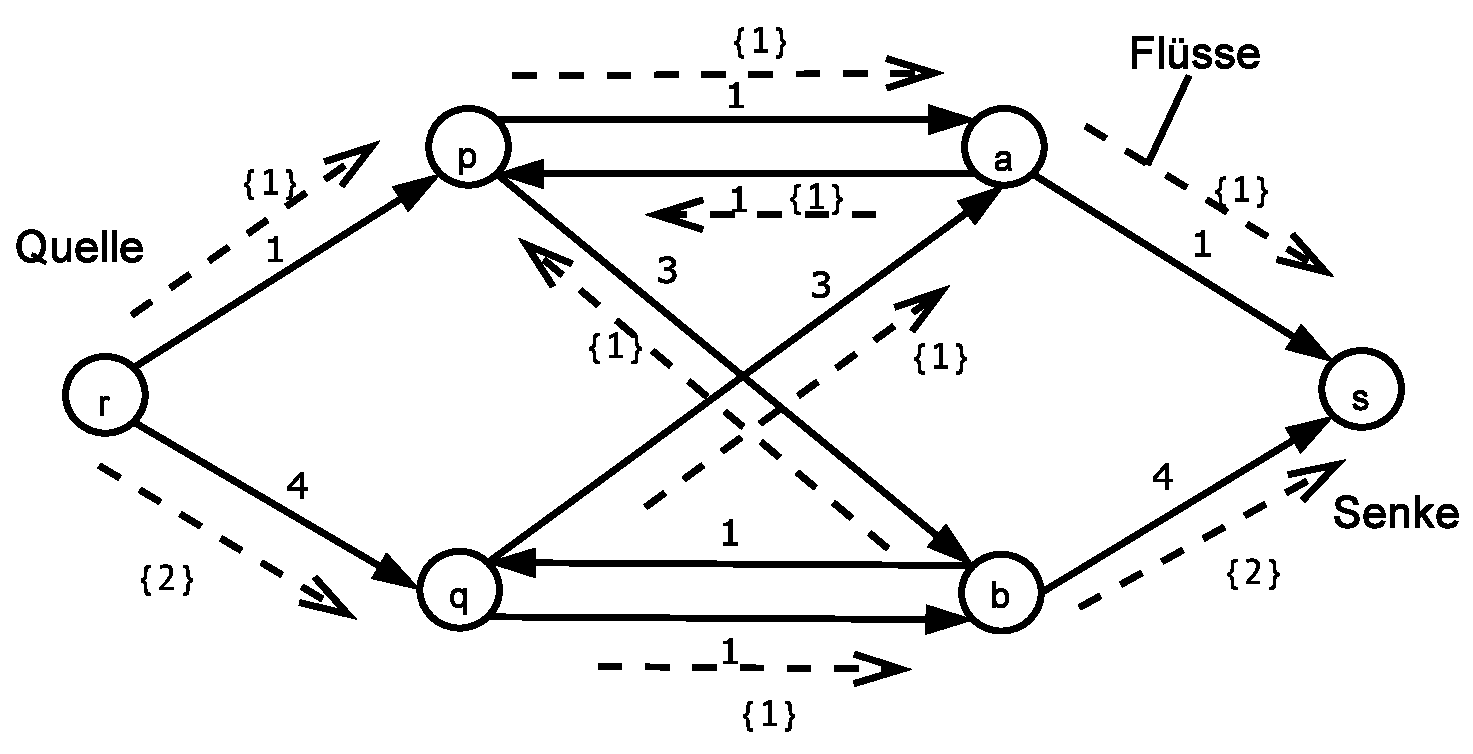
\includegraphics[height=4cm]{bilder/3-0Maxfluss}

Man betrachte den Weg $r,q,a,p,b,s$ und setze Kante $p,a$ zu 0.\\
$\rightarrow$ $p,b$ kann auf 2 gesetzt werden, $b,s$ auf 3, $r,q$ auf 3 und
$q,a$ auf 2.\\
Nun $R=\{r,q,a\}=4$, also ist 4 der optimale Fluss. (Der Schnitt $R$ muss
immer die Quelle enthalten).

Beweis: Mit Korollar \ref{FlussSchnittKap} ist zu zeigen:
\[\exists \mbox{ zul. Fluss x, } \exists \mbox{ Schnitt } \delta(R): \; \;
f_{x} = u (\delta(R))\]
Sei $x$ maximal zulässiger Fluss\\
Def: $R:= \{ v \in V| \exists \mbox{ $x$ erhöhender $(r,v)$-Weg} \}
\hspace{3mm}$ "`$(u\{r\})$"'

Behauptung: $\delta(R)$ ist zugehöriger optimaler Schnitt.\\
Es gilt: $r \in R$, $s \not\in R$ ($x$ optimal)\\
$\forall\;v w \in \delta(R) \; \; \; x_{v w} = u_{v w}$ (sonst
$r\rightarrow\ldots\rightarrow v \rightarrow w$, $x$ erhöhend, aber $w \not\in
R$)\\
$\forall \; v w \in  \delta(\bar{R}) \; \; \; x_{v w} = 0$ (analog).
$\stackrel{\ref{SchnittFluss}}{\Rightarrow} f_{x}(s) = \underbrace{ x
(\delta(R))}_{= u(\delta(R))} -  \underbrace{x (\delta (\bar{R}))}_{=0} =
u(\delta(R))$

\begin{satz}
Ein zulässiger Fluss ist maximal genau dann, wenn kein $x$-erhöhender Weg
existiert.
\end{satz}
Beweis: \\
"`$\Rightarrow$"' klar\\
"`$\Leftarrow$"' Beweis von Satz \ref{MaxFlowMinCut} liefert Schnitt
$\delta(R)$ mit $f_{x}(s) = u (\delta(R)) \stackrel{\ref{FlussSchnittKap}}{
\Rightarrow} x$ ist maximaler zulässiger Fluss. q.e.d.

\begin{satz}
Ist $u$ ganzzahlig und existiert ein maximal zulässiger Fluss, so existiert
ein ganzzahliger maximal zulässiger Fluss.
\end{satz}
Beweis: wähle ganzzahligen maximalen Fluss. $x$ und $u$ ganzzahlig.
$\exists$ x-erhöhender Weg $\Rightarrow \exists$ höherer ganzzahliger Fluss.\\
Einfacher: Existiert ein maximaler zulässiger Fluss so existiert auch der
minimal zulässige Schnitt. Der wiederum setzt sich als Summe der
ganzzahligen Kapazitäten zusammen $\Rightarrow$. Diese Summe ist dann auch 
ganzzahlig.

\begin{korollar}
Ist $x$ ein zulässiger $(r,s)$-Fluss und $\delta(R)$ ein
$(r,s)$-Schnitt, so ist $f_{x}(s)$ Maximum und $u(\delta(R))$ Minimum genau
dann wenn: 
$x_{e} = u_{e} \; \; \forall e \in \delta(R)$\\
$x_{e} = 0 \;\; \forall e \in \delta(\bar{R}) \mbox{ q.e.d.}$
\end{korollar}

\section{Erhöhender Weg (Augmenting Path) Algorithmus}

\begin{algorithmic}
\STATE Starte mit zulässigem Fluss $x$ (z.B. $x=0$)
\WHILE{($\exists x$-erhöhender Weg $P$)}
\STATE $E_{1} := \min \{ u_{e} - x_{e} | e \mbox{ ist Vorwärtskante in
}P\}$
\STATE $E_{2} := \min \{x_{e} | e \mbox{ ist Rückwärtskante in } P \}$
\STATE $E := \min \{E_{1}, E_{2} \}$ \hspace{3mm} "`$x$-Breite von $P$"'
\IF{$(E = \infty)$}
\STATE STOP \hspace{3mm} "`kein maximaler Fluss"'
\ELSE 
\STATE erhöhe Fluss auf $P$ um $E$
\ENDIF
\ENDWHILE
\STATE STOP $x$ maximaler Fluss
$R:= \{v \in V | \exists \mbox{$x$-erhöhender $(r,v)$-Weg} \}$ min Schnitt
$\delta(R)$.
\end{algorithmic}

\subsubsection{Suche nach einem $x$-erhöhendem Weg}
Hilfsdigraph $G(x)$: $V(G(x)) := V$\\
$v w \in E(G(x))$ genau dann wenn $v w \in E$ und $x_{v w} < u_{v w}$ oder $w v 
\in E$ und $x_{w v} > 0$.\\
$(r,s)$-Wege in $G(x) \Leftrightarrow x$-erhöhende Wege in $G$\\
Genannt Breitensuche: Zeit $O(m)$ pro Iteration. Im Beispiel 
(Hilfsdigraph zum ersten Fluss mit Flusswert 3):


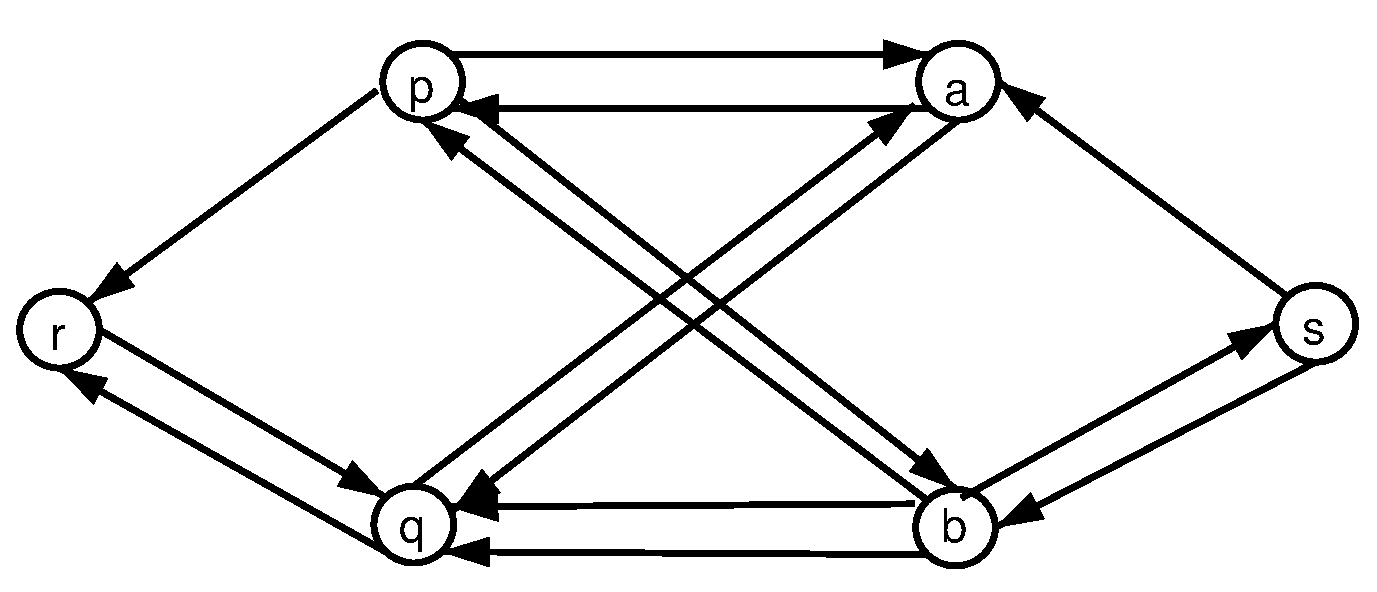
\includegraphics[height=3cm]{bilder/3-0MaxflussDig}

\begin{satz} \label{EW}
Ist $u$ ganzzahlig und der maximale Flusswert $k < \infty$, so terminiert
der erhöhender Wege Algorithmus nach höchstens $k$ Erhöhungen:
\end{satz}
Beweis: $u$ ganzzahlig $\Rightarrow$ alle $x$ ganzzahlig und jede Erhöhung
erhöht den Fluss mindestens um 1. q.e.d.

D.h. für rationale $u$ terminiert der E-W Algorithmus (Skalierung auf ganze
Kapazitäten) - dies gilt also nicht für irrationale Kapazitäten.

Problem:

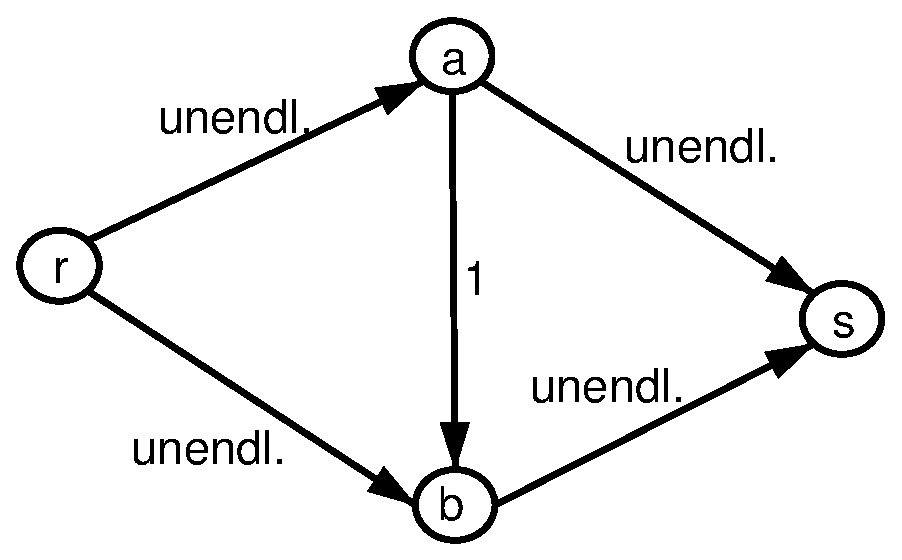
\includegraphics[width=6cm]{bilder/3-0EWTermnicht}

Der Algorithmus wählt immer abwechselnd $r a b s$ und $r b a s \rightarrow$
keine Terminierung wenn $P$ immer über $a b$ geht. Wenn nicht $\infty$
sondern große Zahl $M$, so macht der Algorithmus $M$ Iterationen und hat
einen Fluss von $2M$.\\
$\Rightarrow$ Schranke in \ref{EW} ist scharf

Inputlänge: $n+m+log M$

Ausweg: Kürzeste x-erhöhende, d.h. x-erhöhende Wege mit minimaler
Kantenzahl.

\begin{satz}\label{KEWZeit}
Dinitz [1970], Edmonds und Kasp [1972]\\
Wenn jede Erhöhung auf einem kürzesten, x-erhöhenden Weg statt findet, so
erfolgen höchstens $n \cdot m$ Erhöhungen.
\end{satz}
Beweis: weiter unten nach anderen Sätzen.

\begin{itemize}
\item Keine Annahmen über:
\begin{itemize}
\item Existenz eines maximalen Flusses
\item Rationalität von $u$
\end{itemize}
\item Breitensuche findet einen kürzesten $x$-erhöhenden Weg in Zeit
$O(m)$

Edmonds und Kasp: \begin{quote} "`\ldots so simple that it is likely to be
incorporated innocently into a computer implementation."'
\end{quote}
\end{itemize}

\begin{korollar}\label{ZeitEWA}
Der E-W-Algorithmus mit Breitensuche löst das Max Flow Problem in Zeit
$O(n m^{2})$
\end{korollar}
Zum Beweis von Satz \ref{KEWZeit} zwei Lemmata:

Fluss $x \rightarrow x$-erhöhender Weg $P$ $\underbrace{v_{0}}_{=r}, v_{1},
\ldots, \underbrace{v_{k}}_{=s}$ Fluss $x'$\\
$d_{x}(v,w)$ kürzeste Länge eines $v-w$-Weges in $G(x)$ ($=\infty$ falls
keiner existiert).\\
d.h. $\; d_{x}(r,v_{i}) = i$ \hspace{3mm} $d_{x}(v_{i}, s) = k -i$ $\;\forall\; 0
\leqq i \leqq k$\\
$w v \in E(G(x'))$, $w v \not \in E (G(x)) \Rightarrow (\exists i )\;  w =
v_{i}, \; v = v_{i-1}$

Kante ist jetzt in $G(x')$ da Fluss dort aufgebaut wurde.

\begin{lemma}\label{dxstrichgr}
Für jedes $v \in V$ gilt:
\[d_{x'}(r,v) \geqq d_{x}(r,v)\mbox{ und }d_{x'}(v,s) \geqq d_{x} (v,s)\]
\end{lemma} 
Beweis: Annahme: $(\exists v \in V)\; \; d_{x'}(r,v) < d_{x}(r,v)$\\
Wähle $v$ mit $d_{x'}(r,v)$ Minimum, es gilt $d_{x'} (r,v) > 0 \; \; (v
\not= 0)$\\

Zu $G(x')$: $P'$: $r\underbrace{\rightarrow \; \rightarrow \ldots
\rightarrow}_{\mbox{\scriptsize \begin{tabular}{c}Vorwärts- oder\\
Rückwärtskanten\end{tabular}}}w\rightarrow v$, $w$ ist also der vorletzte Knoten.\\
Länge des Weges $= d_{x'}(r,v)$

Annahme:
\[\begin{array}{rcl}d_{x}(r,v) &>& d_{x'}(r,v)\\
&=&d_{x'}(r,w) + 1 \hspace{3mm} (\ast)\\
&\geqq& d_{x} (r,w) +1 \end{array}\]
$\Rightarrow w v \in E (G(x')) \hspace{5mm} w v \not \in E(G(x))$\\
$\Rightarrow (\exists i ) \; w = v_{i}, \; v=v_{i -1}$\\
$\stackrel{\mbox{\scriptsize$(\ast)$}}{\Leftrightarrow} 
\underbrace{i -1}_{\mbox{
\scriptsize$=$ Distanz von $v=v_{i-1}$}} > \underbrace{i}_{\mbox{
\scriptsize$=$Distanz von $w=v_{i}$}}+1\hspace{3mm}\lightning$\\
$d_{x'}(r,s) \geqq d_{x}(v,s)$ analog q.e.d.

D.h. $\leqq n-1$ Phasen, in jeder Phase: Augmentierungen auf Wegen einer
festen Länge $k$. Frage: Wie oft?
\[E(x):= \{e \in E | e \mbox{ ist Kante eines kürzesten $x$-erhöhenden 
Weges}\}\]

\begin{lemma}\label{KWgroe}
gilt $d_{x'}(r,s) = d_{x}(r,s)$, so gilt $E(x') \subset E(x)$
\end{lemma}
Beweis: Sei $k=d_{x}(r,s) = d_{x'}(r,s)$, $e \in E(x')$\\
$\Rightarrow e = v_{i-1}v_{i}$ oder $e=v_{i}v_{i-1}$ in $x'$-erhöhendem
Weg:
\[P': \; \; \underbrace{\overbrace{v_{0}}^{=v},v_{i},\ldots v_{i-1},}_{
\mbox{\scriptsize$
d_{x'}(r,v)=i-1$}}
\underbrace{v_{i}, \ldots \overbrace{v_{k}}^{s}}_{\mbox{\scriptsize$
d_{x'}(w,s) = k-i$}}\]

$\stackrel{\ref{dxstrichgr}}{\Rightarrow} d_{x}(r,v) + d_{x}(w,s)=k-1$ 

Annahme: $e \not\in E(x) \Rightarrow x_{e} \not= x'_{e} \Rightarrow e \in P
\Rightarrow e \in E(x) \hspace{3mm} \lightning$\\
$\Rightarrow E(x') \subseteq E(x)$

Noch zu Zeigen: $E(x') \neq E(x)$: $\exists e \in P$: $e$ vorwärts und $x'_{e} = u_{e}$ oder $e$ rückwärts und
$x'_{e} = 0$

Annahme: $e \in E(x')$\\
$\Rightarrow$ Jeder $x'$-erhöhende Weg benutzt $e$ anders herum als in
$P$\\
$ (\exists i)$ Länge von $P' > -\underbrace{i}_{\mbox{\scriptsize$r
\ldots v_{i}$}} + \underbrace{k-i+1}_{\mbox{\scriptsize $v_{i-1}\ldots s$}} +
 \underbrace{1}_{v_{i}\ldots v_{i-1}} = k+2 \hspace{3mm}\lightning$\\
$\Rightarrow e \not\in E(x')$

Anschaulich: $e$ ist der Flaschenhals von $P$.

Beweis von Satz \ref{KEWZeit}:\\
Lemma \ref{dxstrichgr} $\Rightarrow$ höchstens $n-1$ Phasen\\
Lemma \ref{KWgroe} $\Rightarrow$ höchstens $m$ Erhöhungen pro Phase\\
$\Rightarrow m n$ Erhöhungen. q.e.d.

D.h. Gesamtlaufzeit für kürzeste erhöhende Wege Algorithmus $O(n m^{2})$.
Später noch ein Algorithmus mit Laufzeit $O(n^{2}m)$.

\section{Anwendungen von Max Flow Min Cut}

\subsection{Bipartite Matchings und Knotenüberdeckungen}
Bipartite Graphen $G(V,E)$ ungerichtet\\
$V=P \cup Q$ \hspace{3mm} $E = \{p q| p \in P, q \in Q\}$\\
$P \cap Q = \varnothing$ \hspace{3mm} $\{P,Q\}$ Bipartition der Graphen.

Bsp:

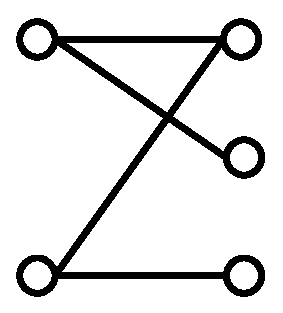
\includegraphics[height=2cm]{bilder/3-0BipMatch}

\paragraph{Bipartites Matching} $M$\\
$M \subseteq E$ mit keine zwei kanten in M haben einen gemeinsamen
Endknoten, b.z.w. $(\forall \; v \in V) | \{ e \in M | v \in e\}| \leqq 1$

Im Beispiel z.B: 

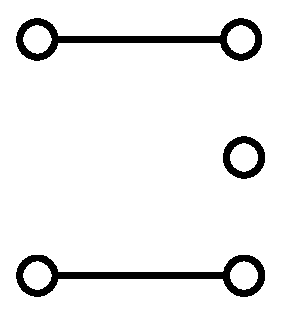
\includegraphics[height=2cm]{bilder/3-0BipMatch2}

\paragraph{Heiratsproblem} \mbox{}\\

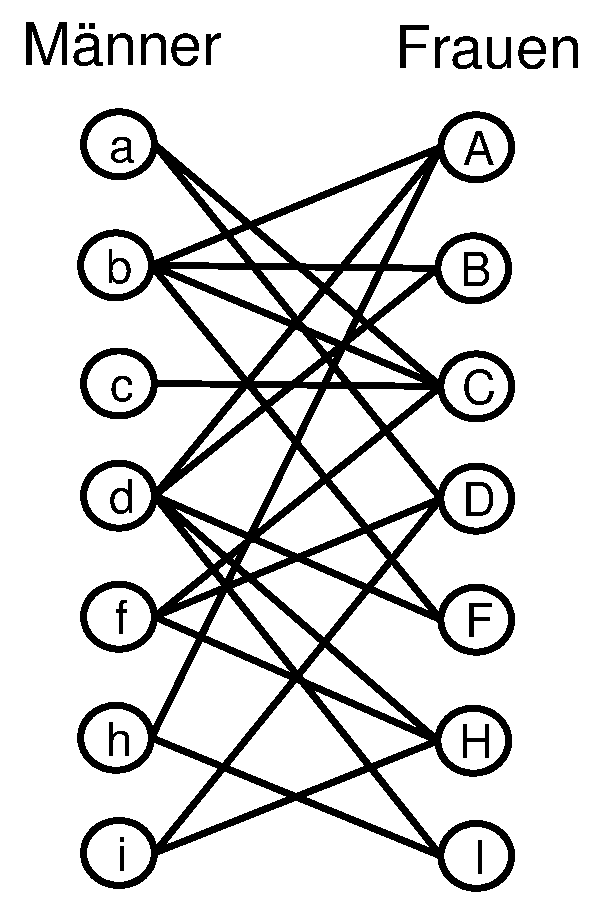
\includegraphics[height=4cm]{bilder/3-0Heiraten}

Hierbei verdeutlichen die Kanten ein "`sich mögen"' und es sollen möglichst
viele Paare verheiratete werden aber nur solche die sich mögen. Eine Lösung
ist:

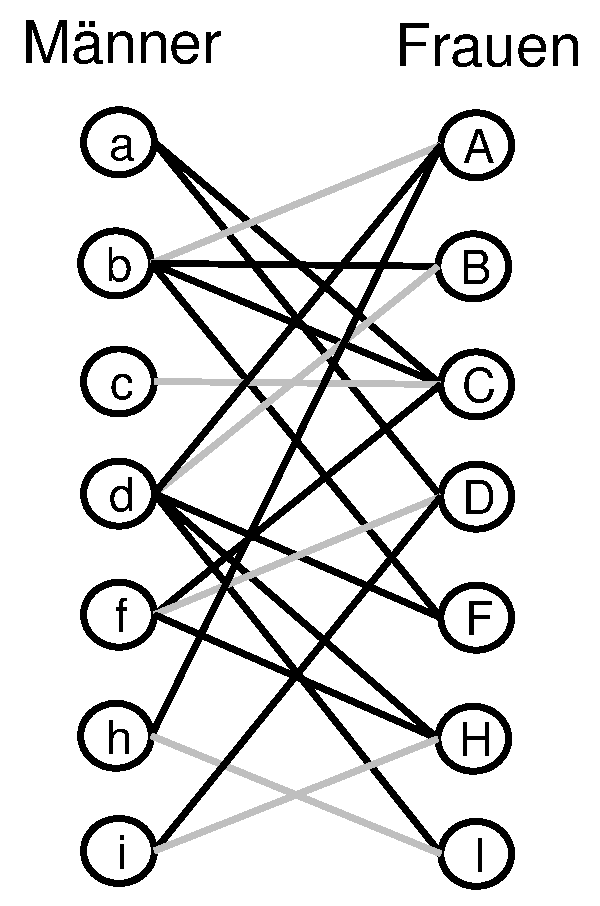
\includegraphics[height=4cm]{bilder/3-0Heiraten2}

Hierbei können also sechs Paare verheiratet werden, wären auch mehr
möglich?

$C \subseteq V$ heißt Knotenüberdeckung falls:
\[ (\forall v w \in E) \; v \in C \mbox{ oder }w \in C\]
Offensichtlich handelt es sich hier um Schwache Dualität.\\
$M$ Matching im bipartiten Graphen $G=(V,E)$\\
$C$ Knotenüberdeckung im bipartiten Graphen $G=(V,E)$\\
$\Rightarrow |M| \leqq |C|$\\

nun die Knotenüberdeckung (grau gefärbte Knoten:)

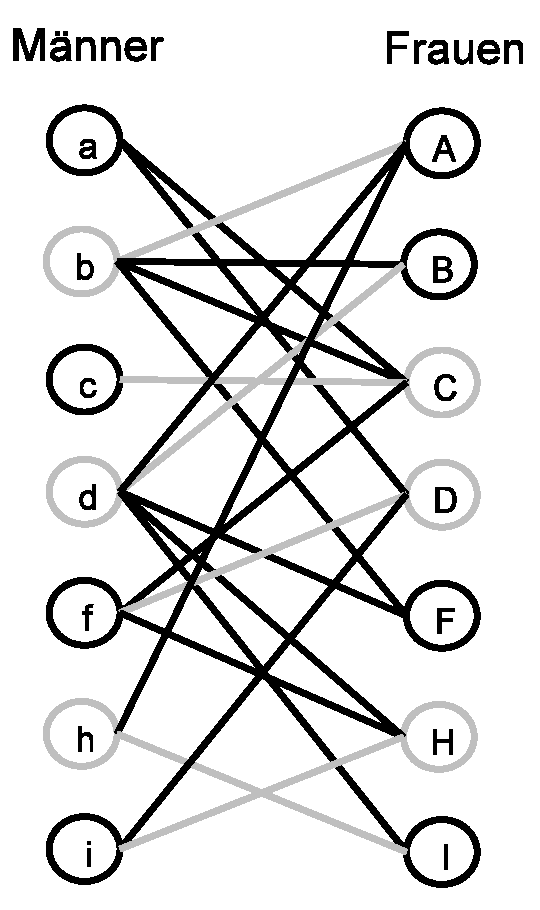
\includegraphics[height=4cm]{bilder/3-0Heiraten3}

Diese hat nun auch 6 Knoten also ist die Lösung auch optimal:\\
$6=\max |M| = \min |C|$

\begin{satz}
Satz von König [1931]\\
Für bipartite Graphen $G=(V,E)$ gilt:\\
\[ \max \{ |M| | \mbox{ ist Matching } \} = \min \{ |C|| \mbox{
ist Knotenüberdeckung } \}\]
\end{satz}
Beweis: Aus ungerichtetem Graphen $G=(V,E)$ konstruieren wir einen
gerichteten Graphen $G'(V',E')$ wie folgt:\\
$ V':= V \cup \{r,s\} \hspace{5mm} E': \forall p q \in E,\; p \in P, q \in
Q$ gerichtete Kanten $p q \in E'$ mit der Kapazität $u_{p q} = \infty$,
zusätzlich $\forall p \in P$ gerichtete Kante $r p$ mit Kapazität $u_{r p}=1$
und $\forall q \in Q$ gerichtete Kante $q s$ mit Kapazität $u_{q s}= 1$

Im Beispiel:

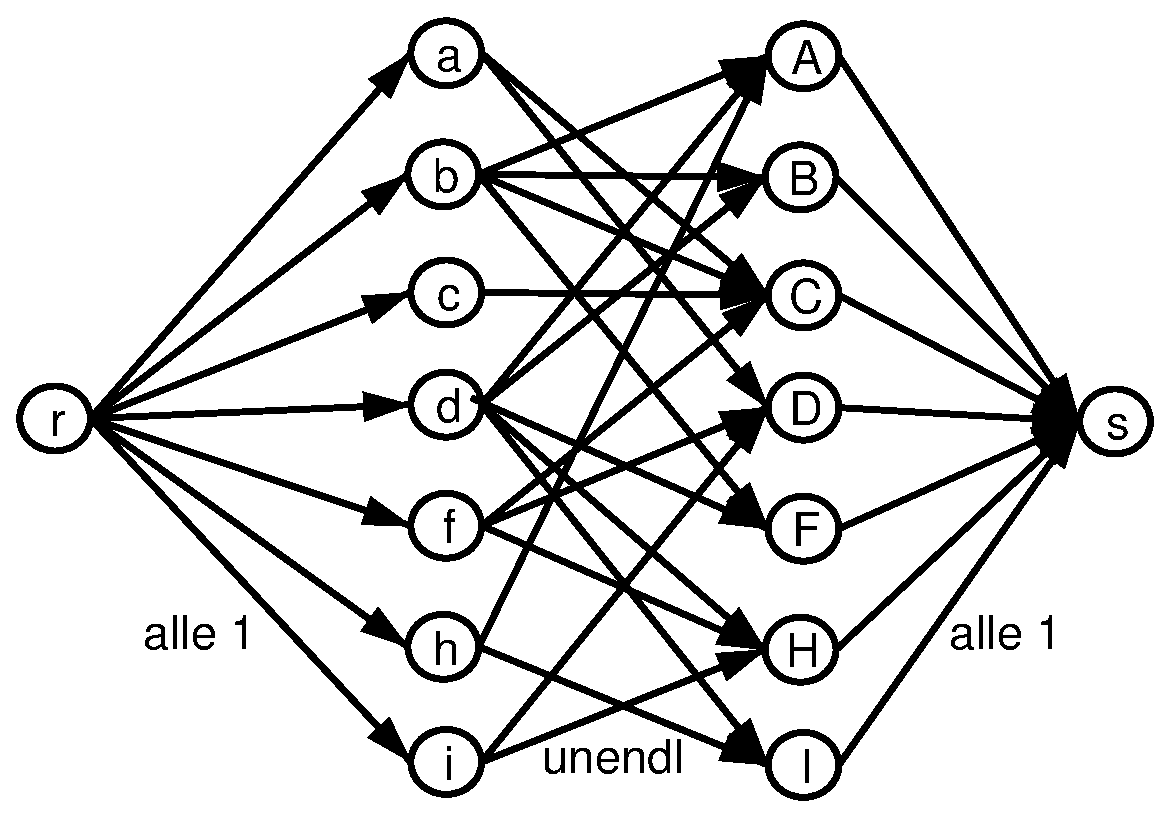
\includegraphics[height=4cm]{bilder/3-0Heiraten4}

Sei $x$ ein ganzzahliger (d.h. 0/1) Fluss in $G'$ mit Flusswert $k$.\\
Wir definieren $M\subseteq E$ durch:
\[\mbox{Für $p q \in E$ gilt } \left\{ \begin{array}{l}
p q \in M \; \mbox{ falls } x_{p q}=1\\
p q \not \in M \mbox{ falls } x_{p q} = 0\\
\end{array} \right.\]
Dann ist $M$ ein Matching in $G$ mit Kardinalität $k$.

Umgekehrt: Sei $M$ ein Matching in $G$ mit Kardinalität $k$.\\
Wir definieren $x_{v w}$ für $v w \in E'$ durch:
\[\begin{array}{ll}
v \in P , \; w \in Q&: x_{v w} = \left\{\begin{array}{l}
1 \mbox{ falls } v w \in M\\
0 \mbox{ falls } v w \not\in M\\
\end{array} \right.\\
v = r, \; w \in P&: x_{v w} = \left\{\begin{array}{l}
1\; (\exists e \in M) \; w \in e\\
0 \mbox{ sonst}\\
\end{array} \right.\\
v \in P, \; w=s&: x_{v w} = \left\{\begin{array}{l}
1\; (\exists e \in M) \; v \in e\\
0 \mbox{ sonst}\\
\end{array} \right.
\end{array}
\]
Dann ist $x$ ein ganzzahliger zulässiger Fluss in $G'$ mit Flusswert $|M|$.

D.h. wir können das maximale Kardinalität Matching mit Max-Flow Berechnung
bestimmen mit höchstens $\min \{|P|,|Q|\} \leqq n$ Flusserhöhungen. Satz
\ref{EW} liefert uns die Laufzeit $O(m n)$ Sei $\delta'(\{r\} \cup A)$ mit
$A \subseteq V$ ein minimaler $(r,s)$-Schnitt in $G'$

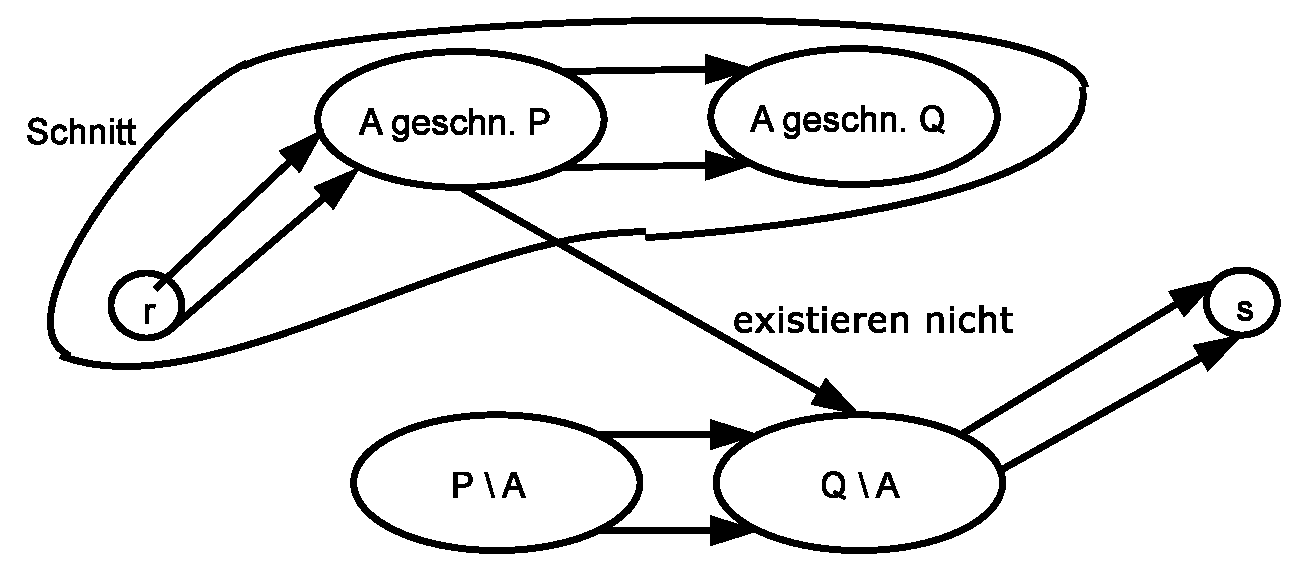
\includegraphics[height=3cm]{bilder/3-0MinKnotenueber}

Endliche Kapazität des Schnitts $\Rightarrow (\nexists v w \in G) \; v
\in  A \cap P, \; w \in Q \wout A$.\\
$\Rightarrow$ Jede Kante $e \in G$ ist inzident zu einem Knoten in $C := (P
\wout A) \cup (Q \cap A)$\\
$\Rightarrow C$ ist Knotenüberdeckung mit Kardinalität $|C| = |P \wout
A| + | Q \cap A| = $ Kapazität des Schnitts $= \max \{|M|| M \mbox{
Matching} \}$\\
D.h. der Algorithmus kann auch eine minimale Knotenüberdeckung berechnen. 

\subsection{Transportproblem}

Gegeben: bipartiter Graph $G=(V,E)$, $V=P\cup Q$, $a\in \ZZ^{P}_{+}$, $b \in
\ZZ^{Q}_{+}$\\
Gesucht: $x \in \RR^{e}$ mit:
\[\begin{array}{rcl}
\displaystyle \sum_{q \in Q, \; p q \in E}x_{p q}&\leqq& a_{p} \; \forall p \in
P\\
\displaystyle \sum_{p \in P, \; p q \in E} x_{p q} = b_{q}\\
x_{p q} &\geqq& 0 \; \forall p q \in E\\
x_{p q}&& \mbox{ganzzahlig } \forall \; p q \in E\end{array}
\]
Nun ist gefragt ob alle Nachfragen $b$ mit den gegebenen Kapazitäten $a$
überhaupt befriedigt werden können. Mathematisch ist also gefragt, ob
eine zulässige Lösung für das Problem existiert. Auch dieses Problem
ähnlich wie das Matching-Problem wird auf ein Max-Flow Problem übertragen:
Beispiel:

\begin{tabular}{c@{\hspace{5mm}}c}
Transportproblem&Flussproblem\\
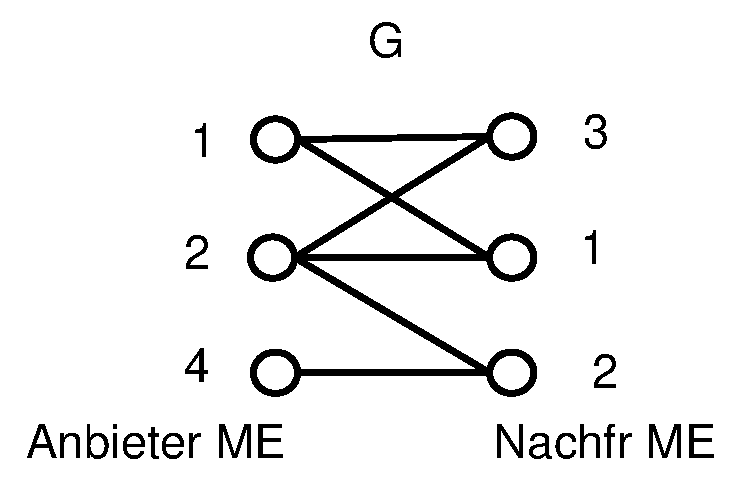
\includegraphics[height=3cm]{bilder/3-0Transport1}&
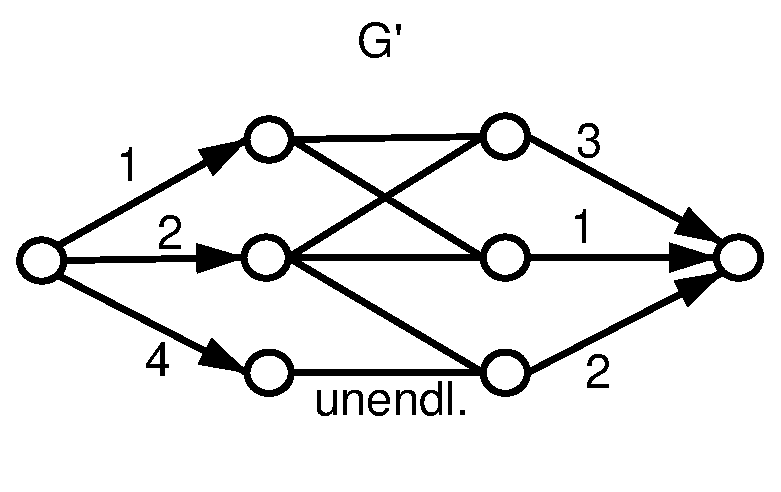
\includegraphics[height=3cm]{bilder/3-0Transport2}\\
$\exists$ Lösung $x\in \ZZ^{E}$ & $\Leftrightarrow \exists$ ganzzahliger
zul. Fluss mit Wert $\displaystyle \sum_{q\in Q} b_{q}$
\end{tabular}

Nach der Umformung kann man einfach den Max-Fluss Algorithmus anwenden:\\
Max-Flow-Min-Cut Theorem:\\
(TB) hat Lösung genau dann wenn jeder $(r,s)$-Schnitt in $G'$ als maximale
Kapazität wenigstens $\displaystyle \sum_{q\in Q} b_{q}$ hat.

Für $A \subseteq P$, $B \subseteq Q$ ist die Kapazität des Schnitts:
\[ \delta'(A\cup B \cup \{r\}) = \sum_{i \in P\wout A} a_{i} +
\sum_{j\in B} b_{j}\]

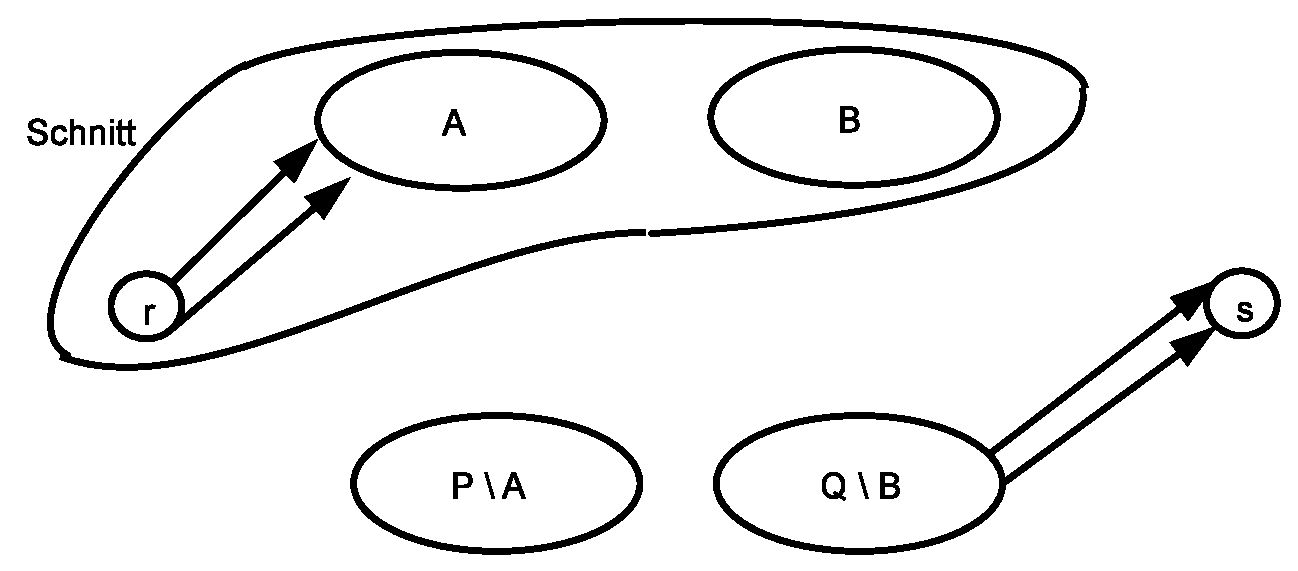
\includegraphics[height=4cm]{bilder/3-0TransportSchnitt}

\[\sum_{i \in P\wout A} a_{i} + \sum_{j \in B} b_{j} \geqq \sum_{q \in Q}
b_q \mbox{ g.d.w. }  \sum_{i \in P \wout A} a_{i} \geqq \sum_{j = Q \wout
B} b_{j}\]
Wir können die Überprüfung beschränken auf solche $A \subseteq P$ für die
gilt: Jeder Knoten aus $P \wout A$ ist mit einem Knoten aus $Q \wout B$
adjazent.

Für $C \subseteq V$:
\[N(C) := \{w \in V | v w \in E \mbox{ für ein v } \in C\} =
(\mbox{ungerichtete Nachbarmenge}) \]
also können wir annehmen:
\[N(Q \wout B) = P \wout A\]
Fazit:
\begin{satz}
$\exists$ Lösung für (TB) genau dann wenn $(\forall \; C \subseteq Q)
\hspace{3mm} a(N(C)) \geqq b(C)$
\end{satz}

Interpretation: Für jede Kundenteilmenge muss der Bedarf durch die
möglichen Produzenten gedeckt sein.

\section{Minimale Schnitte und lineare Optimierung}

Max-Fluss Problem als LP
\[\begin{array}{lrcl}
(LPMF)& \max \displaystyle \sum_{w \in V,\; w s \in E} x_{w s} -
\sum_{w \in V, \; s w \in E} x_{s w}\\
(y_{v})& \displaystyle \sum_{w \in V, \; w v \in E} x_{w v} - \sum_{w \in V,
\; v w \in E} x_{v w}&=& 0 \; \; \forall \; v \in V \wout \{r,s\}\\
(z_{v w})& x_{v w } &\leqq& u_{v w} \; \; \forall \; v w  \in E\\
&x_{v w} &\geqq & 0 \; \; \forall \; v w \in E
\end{array}
\]
Duales LP
\[\begin{array}{lrcl}
(DLPMF)& \min \displaystyle \sum_{v w \in E} u_{v w} z_{v w}\\
&-y_{v} + y_{w} + z_{v w } &\geqq &0 \; \; \forall \; v w \in E, \; v,w \in
V \wout \{r,s\}\\
&y_{w} + z_{r w} &\geqq& 0 \; \; \forall \; r w \in E\\
&-y_{v} + z_{v r} &\geqq& 0 \; \; \forall \; v r \in E\\
&-y_{v} + z_{v s} &\geqq& 1 \; \; \forall \; vs \in E\\
&y_{w} + z_{s w} &\geqq& -1 \; \; \forall \; s w \in E\\
&z_{v w } &\geqq& 0 \; \; \forall \; v w  \in E
\end{array}\]

Vereinfachung durch setzen der neuen Dualvariablen:
\[ y_{r}=0 \hspace{7mm} y_{s} = -1\]
erhalten wir die gemeinsame Form:
\[ -y_{v} + y_{w} + z_{v w} \geqq 0 \; \; \forall \; v w \in E\]

Die Addition von 1 zu allen $y_{v} \; (v \in V)$ ändert die Restriktion
nicht, also ist (DLPMF) äquivalent zu:

\[\begin{array}{lrcl}
(DLPMF')& \min \displaystyle \sum_{v w \in E} u_{v w} z_{v w}\\
&y_{r} &=& 1\\
&y_{s} &=& 0\\
&-y_{v} + y_{w} + z_{v w} &\geqq& 0 \; \;  \forall \; v w \in E\\
&z_{v w} &\geqq & 0 \; \; \forall \; v w \in E
\end{array}\]

\begin{satz}
Falls (DLPMF') eine Optimallösung hat, so hat (DLPMF') eine Optimallösung
 der folgenden Form:\\
Für einen $(r,s)$-Schnitt $\delta(R)$ ist $y$ der charakteristische Vektor
von $R$ und $z$ der charakteristische Vektor von $\delta(R)$
\end{satz}

Beweis:\\
Wähle $\delta(R)$ MIT $r \in R$ als minimalen Schnitt und $y,z$ als die
entsprechenden charakteristischen Vektoren. Dann gilt:

\[ y_{r} = 1, \; \; y_{s} = 0, \; \; z_{v w } \geqq 0 \; \; \forall v w
\in E\]
und:

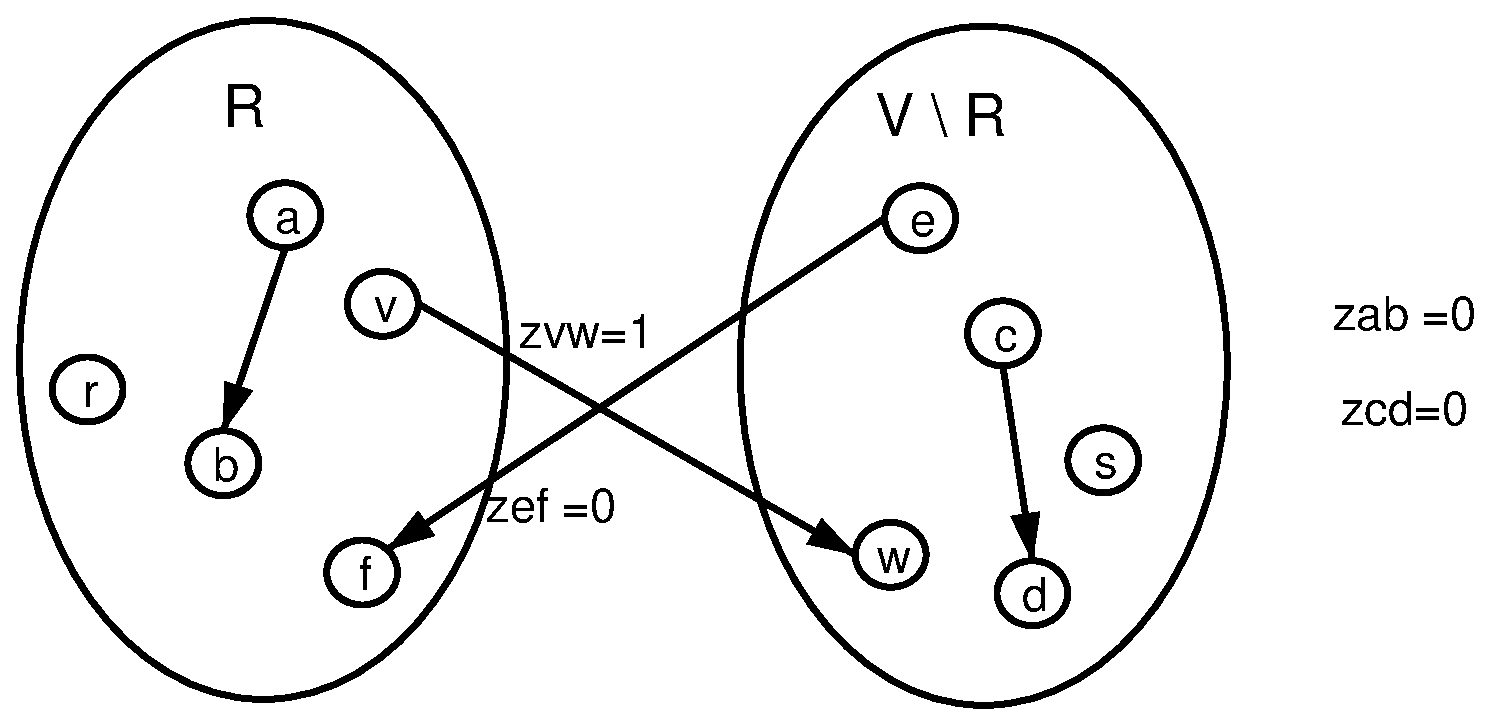
\includegraphics[height=4cm]{bilder/3-0DLPMF}

\[\begin{array}{rcl@{\hspace{5mm}}rcl}-y_{a }- y_{b} + z_{a b}&&&
-y_{c} + y_{d} - z_{c d}\\
-1 + 1 +0 &=&0&=0+0+0&=&0\vspace{2mm}\\
-y_{v}+y_{w}+z_{w}&&&-y_{e}+y_{f}+z_{e f}\\
=-1+0+1&=&0&=0+1+0&>&0\\
\end{array}\]

Somit ist $y_{z}$ zulässig für (DLPMF') und der ZF-Wert ist:

\[\begin{array}{rcl}
\displaystyle \sum_{v w \in E} u_{v w} z_{v w } &=& u(\delta(R))\\
&\stackrel{\mbox{\scriptsize Max-Flow-Min-Cut}}{=}&\mbox{Wert des max.
Flusses}\\
&=& \mbox{Optimaler Wert (LPMF)}\\
&\stackrel{\mbox{\scriptsize Dualitätsth.}}{=}& \mbox{Optimaler Wert von
(DLPMF')} 
\end{array}\] 

\subsubsection{Formulierung des minimalen Schnitt Problems ohne y-Variable}

\[\begin{array}{rrcl}
(LPMC)\hspace{7mm}& \min \displaystyle \sum_{e \in E} u_{e} z_{e}\\
\mbox{s.t.}& \displaystyle \sum_{e\in P} z_{e} &\geqq& 1 \; \; \forall \;
\mbox{einfache $(r,s)$-Wege $P$}\\
&z_{e} &\geqq&0 \; \; \forall \; e \in E \end{array} 
\]
Offensichtlich: Jeder charakteristische Vektor eines $(r,s)$-Schnittes
$\delta(R)$ $z_{e}=\left\{ \begin{array}{l}\mbox{1 falls $e \in \delta(R)$}\\
\mbox{0 sonst}\end{array}\right.$ ist zulässig für (LPMC).
\begin{satz}
Falls (LPMC) eine Optimallösung hat, so hat (LPMC) eine Optimallösung, die
charakteristischer Vektor eines $(r,s)$-Schnittes ist.
\end{satz}
Beweis: Wäre $u_{e} < 0$ für ein $e \in E$, so wäre (LPMC) unbeschränkt,
also gilt: $u_{e} \geqq 0 \; \forall \; e \in E$\\
Sei $z'$ charakteristischer Vektor eines minimalen $(r,s)$-Schnittes
$\delta(R)$. Das duale LP lautet:
\[\begin{array}{rrcl}
(DLPMC)\hspace{7mm}& \max \displaystyle \sum_{P \mbox{ einf. $(r,s)$-Weg }}
w_{P}\\
\mbox{s.t.}&\displaystyle \sum_{P} w_{P} &\leqq & u_{e} \; \; \forall \; e \in E\\
&w_{P} &\geqq & 0 \; \; \forall \mbox{ einf. $(r,s)$-Wege } P \end{array}
\]
Sei $x$ ein maximaler Fluss mit Wert $F$.\\
Wiederhole:\\
Finde einfachen $(r,s)$-Weg $P$ der Form:
\[r\stackrel{x_{e_{1}}>0}{\longrightarrow}\bullet
\stackrel{x_{e_{2}}>0}{\longrightarrow}\bullet\longrightarrow \ldots
\stackrel{x_{e_{k-1}}>0}{\longrightarrow}\bullet
\stackrel{x_{e_{k}}>0}{\longrightarrow}s\]
Setze $w_{p} := \min\{x_{e_{i}} | 1 \leqq i \leqq k\}$\\
Setze für $1 \leqq i \leqq k: \; x_{e_{i}} := x_{e_{i}} -w_{p}$ bis $f_{x} = 0$. Nun gilt $\displaystyle \sum_{P} w_{p} = F$\\
Die Prozedur terminiert, da immer wenigstens ein $x_{e}$ Null wird.\\
$w$ ist zulässig für (DLPMC) und 
\[\sum_{P} w_{p} = \sum u_{e} z'_{e}\]
$\Rightarrow z'$ ist optimal für (LPMC)

\section{Der Algorithmus von Goldberg und Tarjan [1988]}
Vereinbarung: Falls $v w \in E$ und $ w v \not\in E$ setzen wir $u_{w v} =
x_{w v}=0$ (nur für Beschreibung des Algorithmus, die Implementierung fügt
Kante nicht hinzu).

Für $x \in R^{e}$ (nicht notwendigerweise Fluss) mit $0 \leqq x_{e} \leqq
u_{e} \; \forall \; e \in E$ definieren wir den Hilfsdigraphen $G(x)$.\\
$v w \in E(G(x)) \Leftrightarrow x_{v w} < u_{v w}$ oder $x_{w v} > 0$.
Parallele Kanten in $G(x)$ sind nicht erlaubt.

Restkapazität von $v w$: $\bar{u}_{v w} := u_{v w } - x_{v w} + x_{w v}$\\
($\bar{u}_{v w}$ kann auf $v w$ zusätzlich fließen ohne $0 \leqq x_{v w}
\leqq u_{v w}$ zu verletzen. Eine solche Lösung verletzt im Allgemeinen aber
die Flusserhaltungsbedingung)

$x$ heißt Präfluss (Preflow) falls:
\[f_{x}(v) \geqq 0 \; \; \forall \; v \in V \wout \{r,s\}\]

\paragraph{Push Operation} für $v w \in E$ mit $\bar{u}_{v w} > 0$ und
$f_{x}(v)>0$ 
\[x_{v w}\ \leftarrow x_{v w} + \underbrace{\min (\bar{u}_{v w},\; f_{x}(v))
}_{:= \epsilon}\]
Erhält die "`zulässiger Präfluss"' Eigenschaft. (Falls auch $w v \in E$ und
$\epsilon < \bar{u}_{v w })$\\
\[\begin{array}{rcl}
x_{w v} &\leftarrow& x_{w v} - \underbrace{\min(\epsilon, \; x_{w v})}_{ :=
\epsilon'}\\
x_{v w} &\leftarrow & x_{v w} + \epsilon - \epsilon'\end{array}
\]

Beispiel:

\begin{tabular}{l}
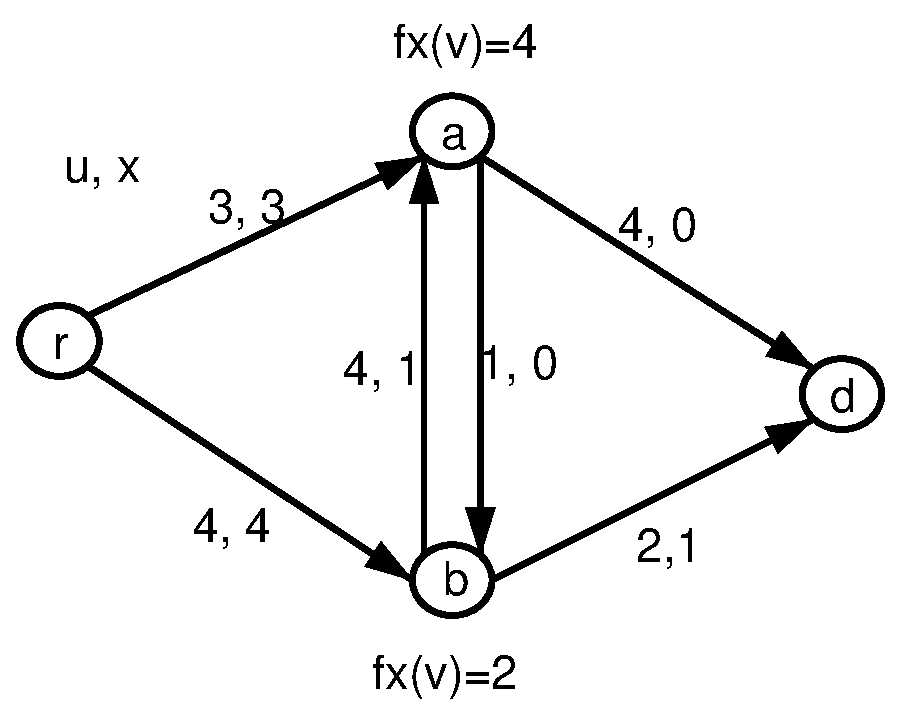
\includegraphics[height=3cm]{bilder/3-0Praefluss1}
\end{tabular}
$\stackrel{\mbox{push}(a,b)}{\Longrightarrow}$
\begin{tabular}{l}
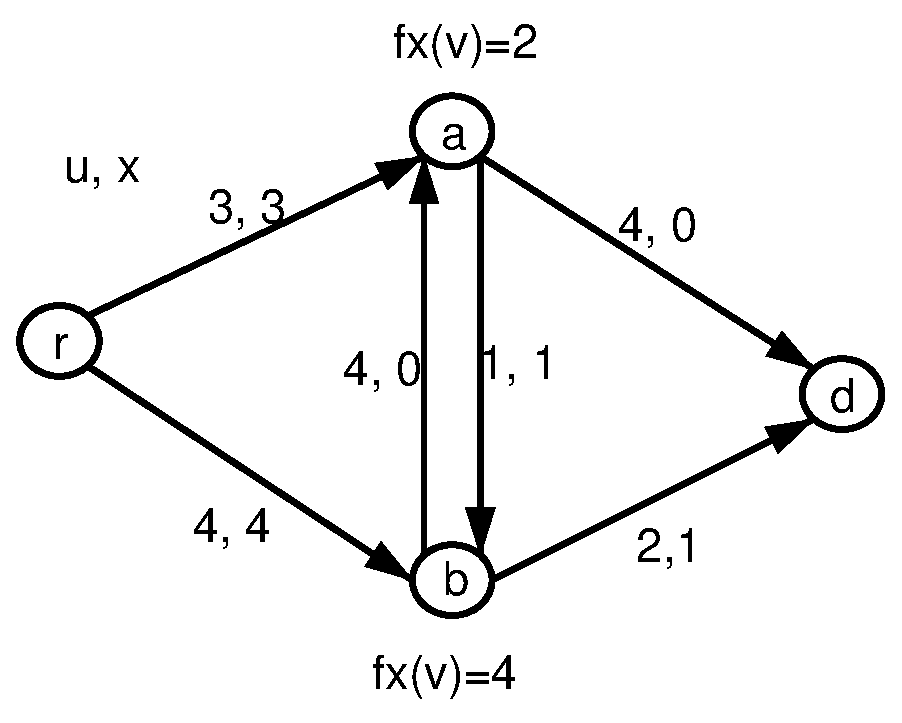
\includegraphics[height=3cm]{bilder/3-0Praefluss2}
\end{tabular}


Zu erkennen ist dass hier auch die "`zulässiger Präfluss"' Eigenschaft
erhalten bleibt.\\
Knoten $v \in V \wout \{r,s\}$ ist {\em aktiv} falls $f_{x}(v) > 0$\\
$\Rightarrow$ Ein Präfluss ist ein Fluss, falls es keine aktiven Knoten
gibt.

Grundoperationen:
\begin{enumerate}
\item Wähle einen aktiven Knoten $v$
\item Wähle $v w \in G(x)$
\item push $v w$
\end{enumerate} 
Wesentlich ist die richtige Reihenfolge, sonst könnte der Algorithmus
unendlich operieren: push$(v w)$, push$(w v)$, push$(v w)$, push$(w v),
\ldots$

$d \in (\ZZ^{+} \cup \{\infty\})^{V}$ ist eine gültige Nummerierung (valid
labeling) bezüglich eines Präflusses $x$ falls:
\[\begin{array}{rcl}
d(r)&=&n\\
d(s)&=& 0\\
d(v) &\leqq& d(w) +1 \; \; \forall \; v w \in G(x)  
\end{array}\]

Invariante des GT-Algorithmus: Zulässiger Präfluss mit gültiger Nummerierung.

{\bf Initialisierung:}\\
Initialisiere $(x,d)$;\\
$\forall \; i j \in E$ setze  $x_{i j} = \left\{ \begin{array}{l}u_{i j}, \mbox{
falls } i=r\\ 0 \mbox{ sonst}\end{array} \right.$\\
$\forall \; i \in V$ setze $d_{i} = \left\{ \begin{array}{l}n, \mbox{
falls } i=r\\ 0 \mbox{ sonst}\end{array} \right.$

$x$, $d$ erfüllen gültige Nummerierung (wir müssen annehmen, dass alle
$u_{r v} < \infty$ falls nicht, so kann man diese Bedingung herstellen. In
der Übungsaufgabe...)

Beispiel:

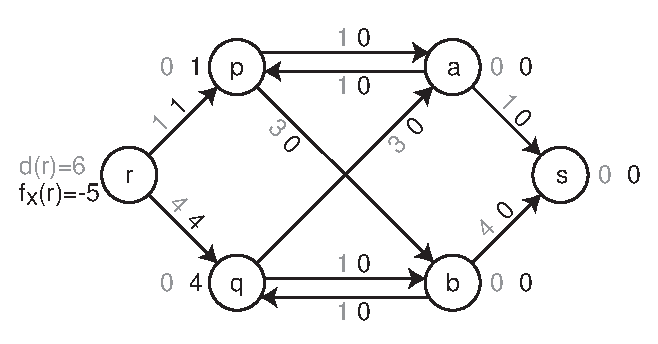
\includegraphics[height=4cm]{bilder/3-0GoldbTarjan}

\begin{lemma}
Ist $x$ ein zulässiger Präfluss und $d$ eine gültige Nummerierung bezüglich
$x$, so existiert ein $(r,s)$-Schnitt $\delta(R)$, so dass\\
\[\begin{array}{rcl}
x_{v w}&=& u_{v w} \; \; \forall \; v w \in \delta(R)\\
x_{v w}&=& 0 \; \; \forall \; v w \in \delta(\bar{R})
\end{array}\]
\end{lemma}
Beweis: In einer gültigen Nummerierung $\exists k, \; 0 < k < n, \; d(v)
\not= k \forall \; v \in V$ ($n-1$ Zahlen auf $n-2$ Knoten, einer bleibt
über)\\
Setze $R:= \{v \in V | d(v) > k\}$\\
dann ist $r \in R, \; s \not\in R$ und wegen gültiger Nummerierung kann
keine Kante in $G(x)$ $R$ verlassen $\Rightarrow$ Behauptung.

\begin{korollar}\label{GueltmaxFluss}
Hat ein zulässiger Fluss eine gültige Nummerierung, so ist $x_{e}$ ein
maximum Fluss.
\end{korollar}
Korollar \ref{GueltmaxFluss} liefert Terminierungsbedingung.
Invariante:
\begin{enumerate}
\item zulässiger Präfluss
\item gültige Nummerierung (d.h. saturierter Schnitt)
\end{enumerate} 
Terminierung sobald Fluss.

vgl. Erhöhender Wege-Algorithmus:
Invariante:
\begin{enumerate}
\item zulässiger Fluss
\item Terminierung, sobald ein Schnitt saturiert ist.
\end{enumerate}
Die gültige Nummerierung approximiert Distanzen in $G(x)$
\begin{lemma}
Für jeden zulässigen Präfluss $x$ und jede gültige Nummerierung $D$
bezüglich $x$ gilt:
\[d_{x}(v,w) \geqq d(v) - d(w) \; \; \forall v, w \in V\]
\end{lemma}
Beweis: für $d_{x}(v,w) = \infty$ trivial.\\
für $d_{x}(v,w) < \infty$, $P$ ein kürzester gerichteter (v,w)-Weg in
$G(x)$.\\
Wir addieren die Ungleichungen $d(p) - d(q) \leqq 1$ für alle $p q \in P$.
\\ Summe: $d(v) - d(w)$ q.e.d.

Insbesondere gilt:
\[\begin{array}{rcl}d(v) &\leqq& d_{x}(v,s)\\
d(v)-n &\leqq & d_{x}(v,r)\end{array}\]
Also $d(v) \geqq n \Rightarrow d_{x}(v,s) = \infty$\\
D.h. in diesem Fall sollte der Fluss Richtung Quelle "`gepusht"' werden.

\paragraph{Strategie}: $push(v w)$ mit $d(w) < d(v)$\\
\[\left.\begin{array}{l}
\mbox{gültige Nummerierung}\\
v w \in G(x)\\
d(w) < d(v)\end{array} \right\}\rightarrow d(w) = d(v) -1\]
$v w$ eine {\em zugelassene Kante} (admissible arc) falls $v w \in E(G(x)), d(v) =
d(w) +1$\\
Ein $push(v w)$ auf $v w$ erhält die gültige Nummerierung. $w v$ könnte in
$E(G(x'))$ sein, aber $d(w) \leqq d(v)+1$ gilt bereits vorher.

Was ist aber nun wenn $v$ aktiv ist aber $(\nexists v w \in G(x)) \; d(v) =
d(w) +1$? Antwort: $relabel(v)$: $d(v) \leftarrow min\{d(w) +1| v w \in
E(G(x))\}$.

Auch danach ist die Nummerierung in $G(x)$ noch gültig:

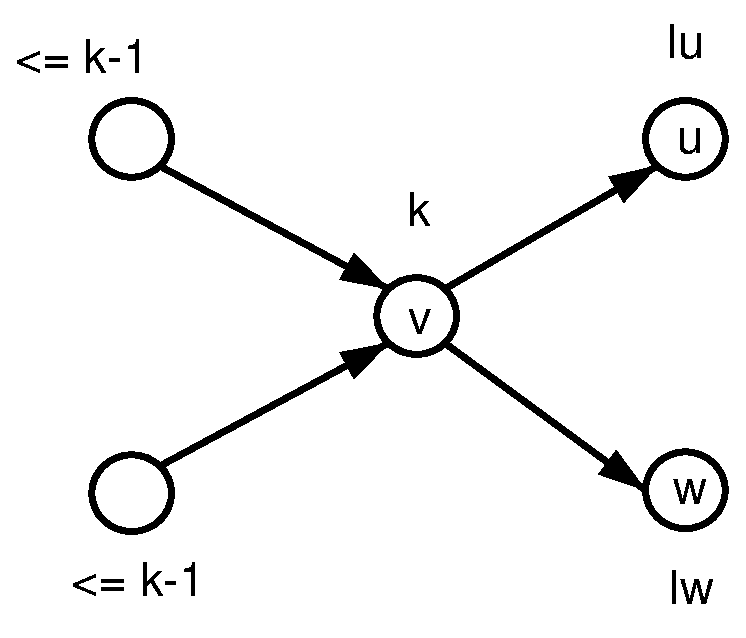
\includegraphics[height=3cm]{bilder/3-0PushOp}
\\$\begin{array}{l}l_{u} \geqq k -1\\
\mbox{hier: }l_{u}\ \geqq k\\
l_{w} \geqq k -1\\
\mbox{hier: }l_{w}\geqq k\end{array}$

Wenn $l_{w}$ Minimum ist, dann erhält $v$ also die Nummer $l_{w}+1$

$process(v)$
\begin{algorithmic}
\WHILE{$\exists$ zugelassene Kante $v w$}
\STATE $push(v w)$;
\IF{$v$ aktiv}
\STATE $relabel(v)$
\ENDIF
\ENDWHILE
\end{algorithmic}

\paragraph{Der Goldberg-Tarjan Algorithmus} \mbox{}\\
\begin{algorithmic}
\STATE initialize $(x,a)$;
\WHILE{$x$ is not a flow}
\STATE choose active node $v$;
\STATE $process(v)$
\ENDWHILE
\end{algorithmic}

Beispiel: Wir wählen immer $v$ mit größter Distanz $d(v)$ "`maximum
distance"'-Version des GT-Algorithmus. 
%Vielen Dank an Prof. Jünger dafür,
%dass er freundlicherweise Scans der Zeichnungen zur Verfügung gestellt hat.
Vielen Dank an Daniel Teske für die Zeichnungen...

An den Knoten sind die grauen Zahlen die Distanzlabel, die dunklen
Nettofluss/Überschuss, an den Kanten sind die Kapazitäten hell und der
Fluss dunkel.

%\begin{tabular}{ccc}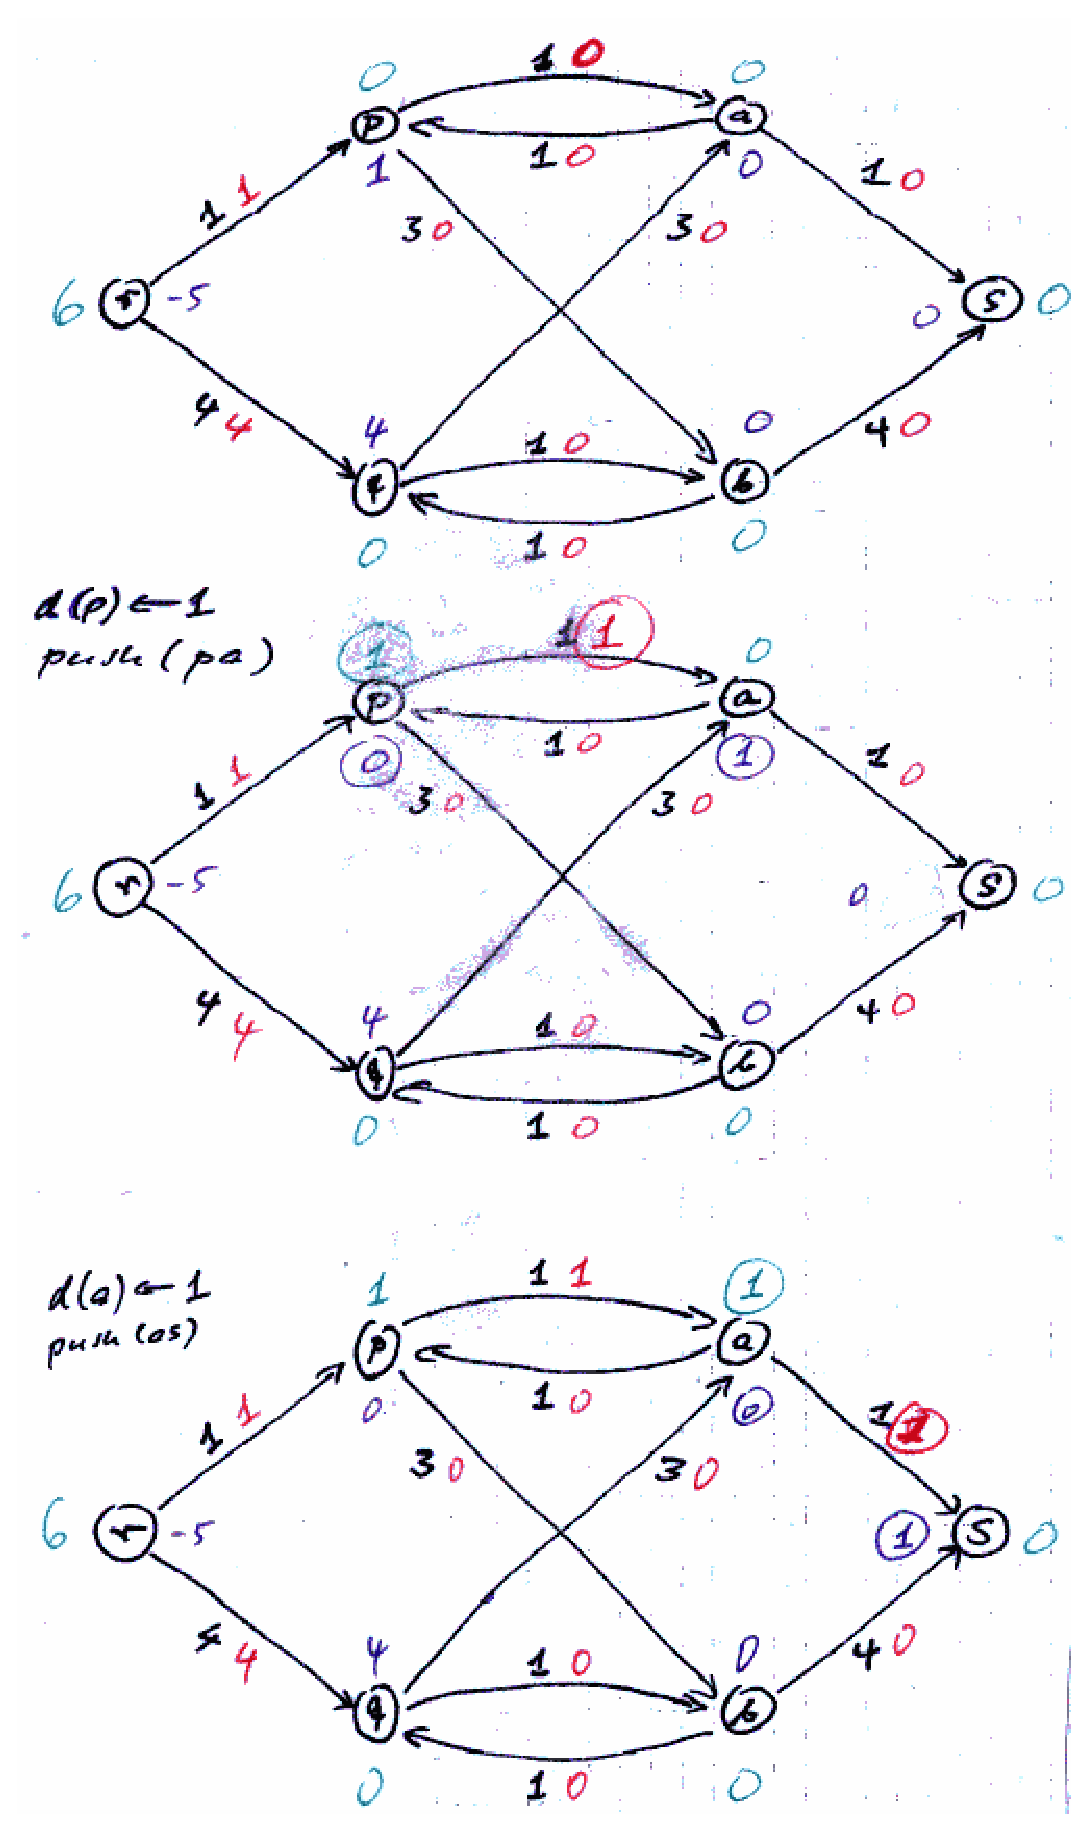
\includegraphics[width=5cm]{bilder/3-0Tarjan1}
%&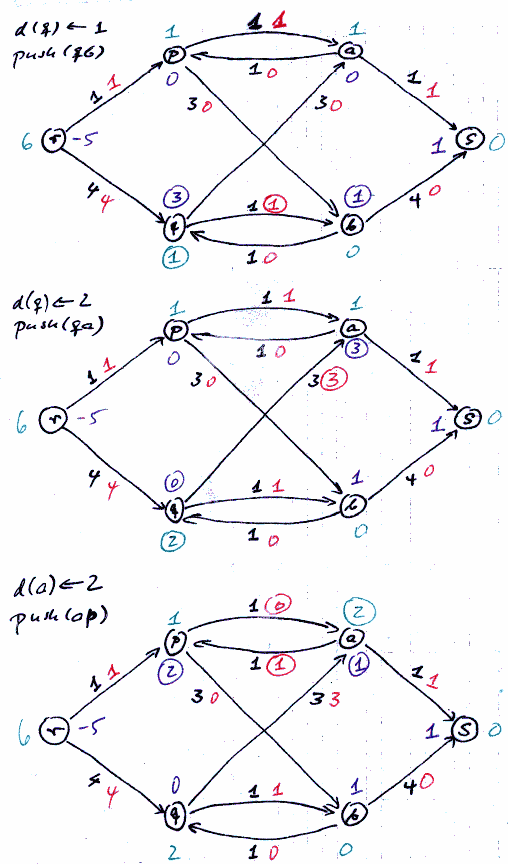
\includegraphics[width=5cm]{bilder/3-0Tarjan2}
%&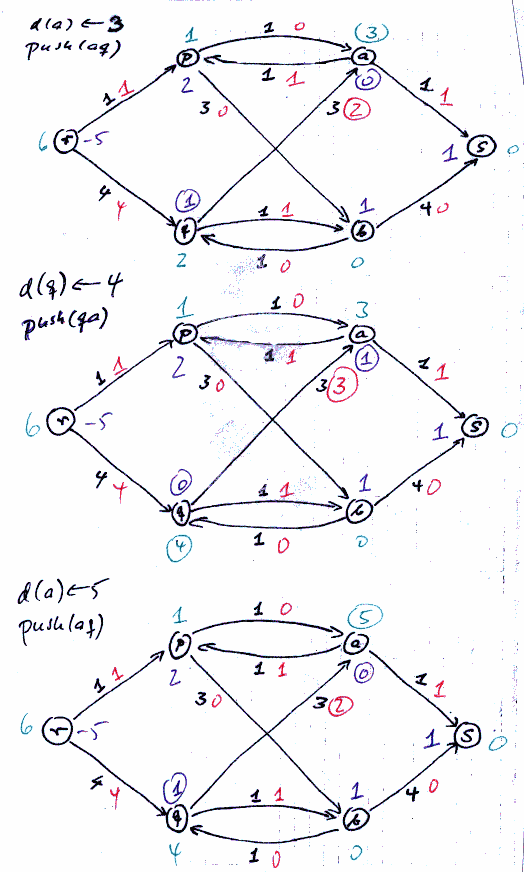
\includegraphics[width=5cm]{bilder/3-0Tarjan3}\end{tabular}

%\begin{tabular}{cc}
%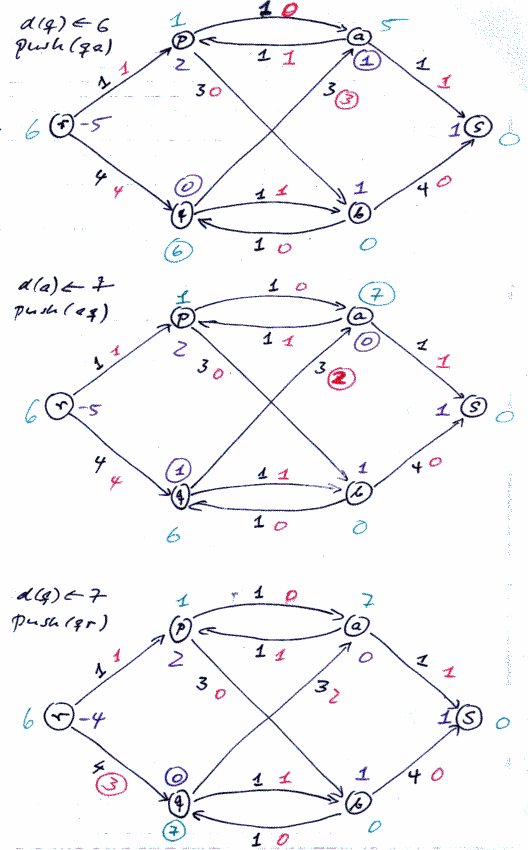
\includegraphics[width=5cm]{bilder/3-0Tarjan4}&
%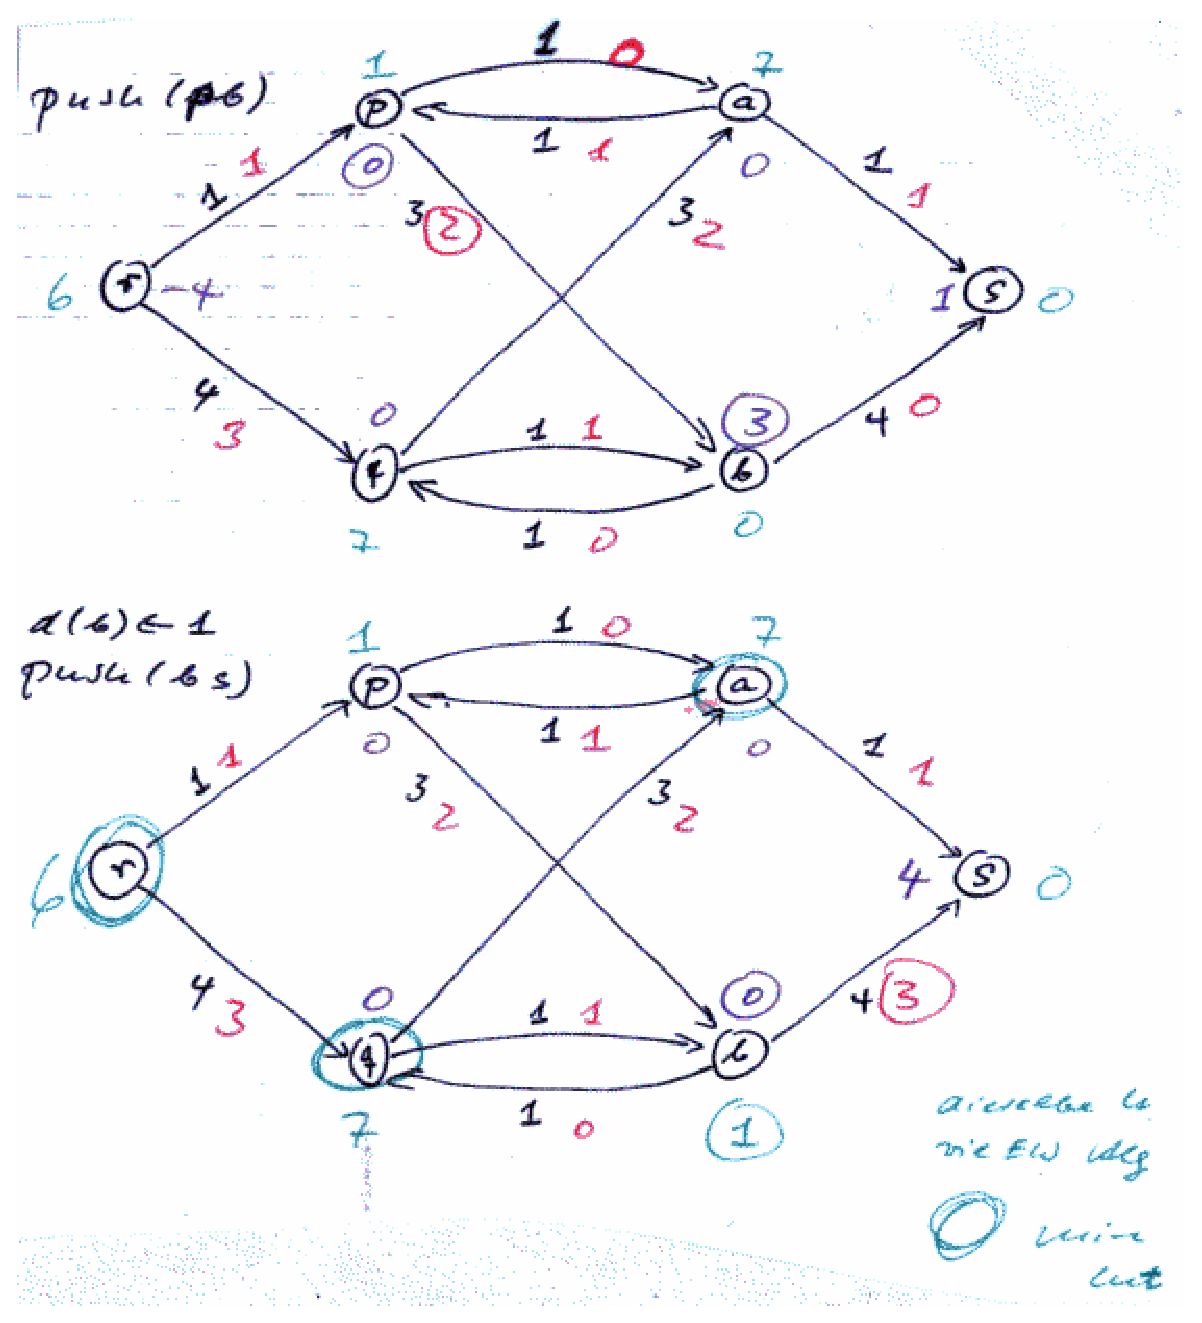
\includegraphics[width=5cm]{bilder/3-0Tarjan5}\end{tabular}

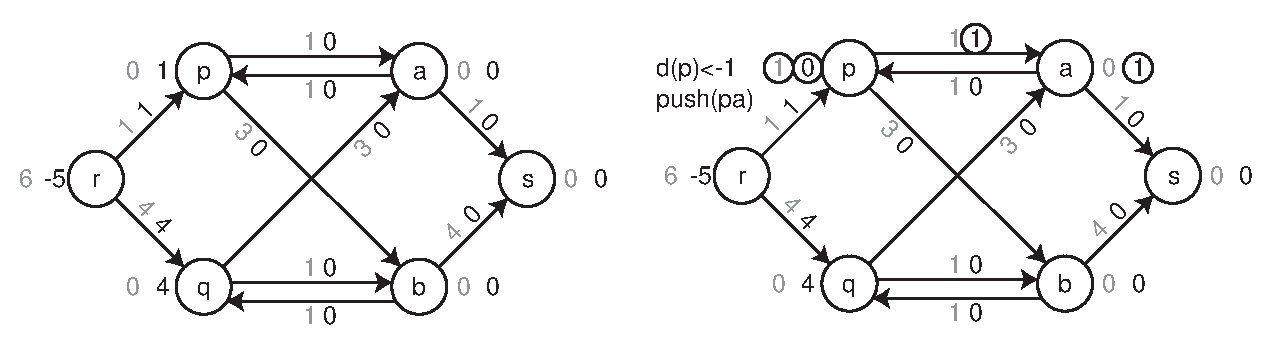
\includegraphics[width=15cm]{bilder/3-0GBTarjan1}

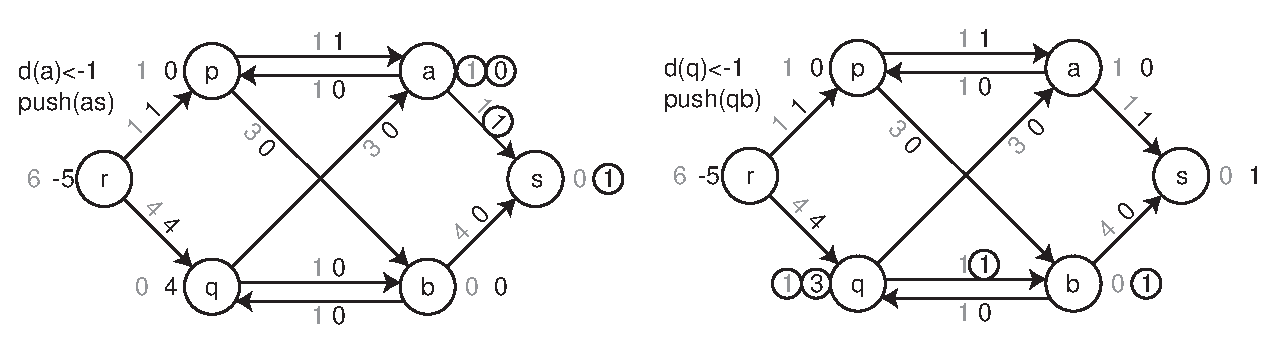
\includegraphics[width=15cm]{bilder/3-0GBTarjan2}

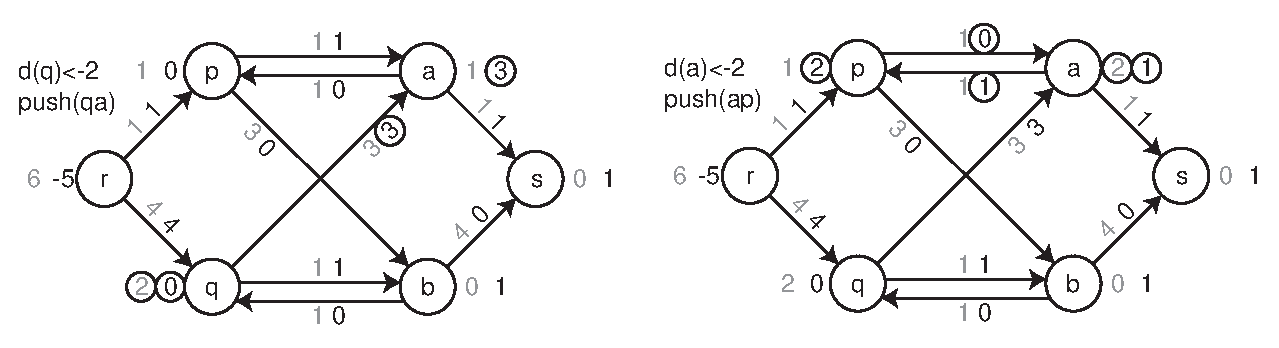
\includegraphics[width=15cm]{bilder/3-0GBTarjan3}

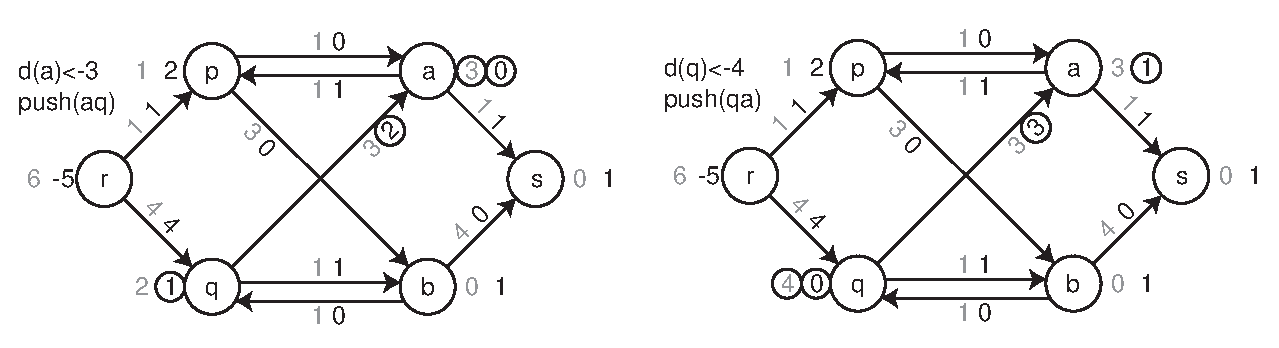
\includegraphics[width=15cm]{bilder/3-0GBTarjan4}

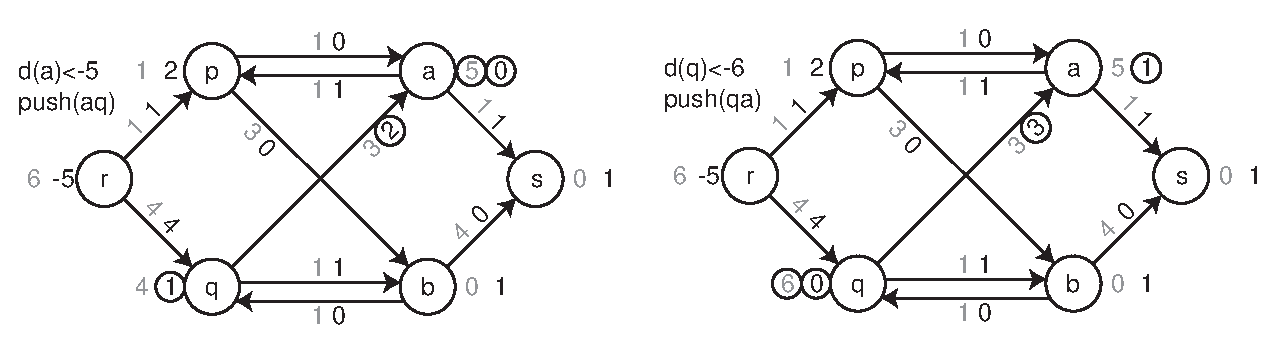
\includegraphics[width=15cm]{bilder/3-0GBTarjan5}

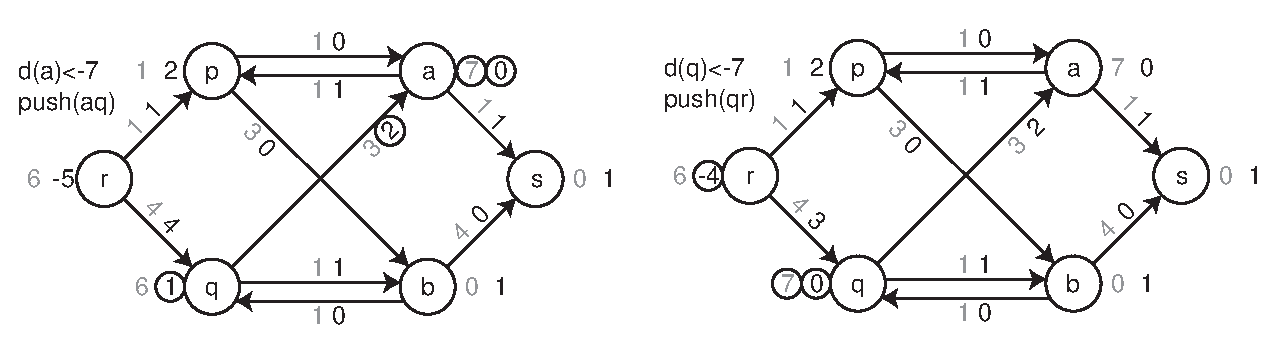
\includegraphics[width=15cm]{bilder/3-0GBTarjan6}

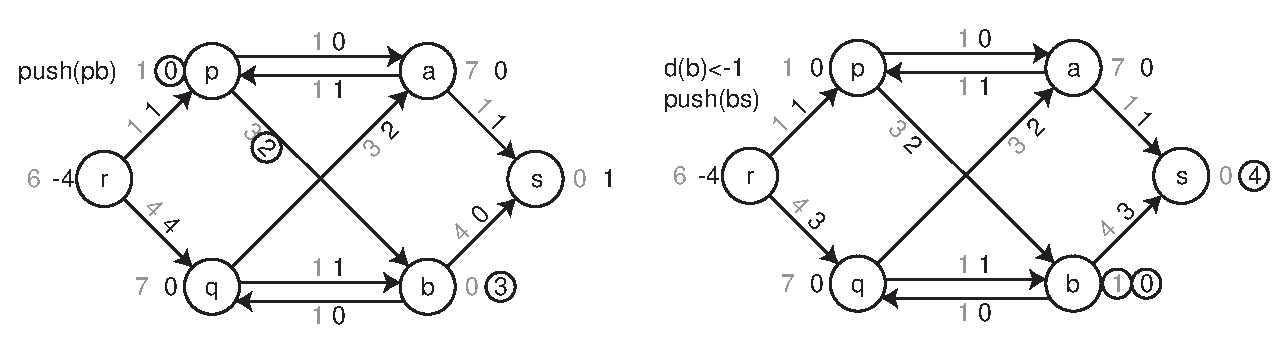
\includegraphics[width=15cm]{bilder/3-0GBTarjan7}


\begin{satz}
Der (max-distance) GT-Algorithmus ist korrekt. Der GT-Algorithmus führt
$O(n^{2})$ relabel Operationen durch, sowie $O(n^{2}m)$ push-Operationen in
der Urversion und $O(n^{2}\sqrt{m})$ in der max-dist-Version.

Die Urversion kann so implementiert werden, dass sie $O(n^{2}m)$ Zeit
benötigt, die max-dist-Version so, dass sie $O(n^{2}\sqrt{m})$ Zeit
benötigt.
\end{satz}
Beweis: Korrektheit folgt aus Korollar \ref{GueltmaxFluss}: Falls
GT-Algorithmus terminiert, so mit einem maximalen Fluss.

Die Laufzeit ist sehr aufwendig zu beweisen, deswegen verzichten wir an
dieser Stelle darauf.

Aus der Praxis kann man sagen das der GT-Algorithmus dort gute Ergebnisse
erzielt.

\section{Minimale Schnitte in ungerichteten Graphen ("`Min-Cut"')}

Gegeben: ungerichteter Graph $G=(V,E)$ mit Kantenkapazitäten $z_{e} \geqq 0
\; \; \forall \; e \in E$.

Gesucht: $\varnothing \neq S \subset V$ mit $z(\delta(S))$ Minimum.\\
Dieses Problem tritt z.B. als Teilproblem des TSP auf.

Spezialfall: $z_{e} = 1 \forall \; e \in E$: Bestimmung des
Knotenzusammenhangs. (minimale Anzahl von Kanten die entfernt werden müssen
um $G$ unzusammenhängend zu machen).

Sei $G$ zusammenhängend (sonst ist es trivial), z.B. Breitensuche findet in
Linearzeit ein $S$ mit $z(\delta(S))=0$. Das Problem kann
offensichtlich via ${n \choose 2}$ $(r,s)$-Max Flow-Min-Cut Berechnungen
gelöst werden. $\rightarrow$ Laufzeit $O(n^{5})$

\paragraph{Schrumpfen eines Knotenpaares $i,j \in V$} \mbox{} \\
\begin{enumerate}
\item $V \leftarrow V \wout \{ i,j\} \cup \{p\}\; \; \; $ $p$ ist also 
neuer Knoten.
\item Ersetze in $p$ jedes Paar von Kanten
\[e'=i k \hspace{5mm} e''= j k\]
durch:
\[e^{\ast} = p k \mbox{ mit } z_{e}^{\ast} = z_{e'} + z_{e''}\]
\item Ersetze in $E$ alle Kanten $i e$ durch $p e$ mit $z_{p e} = z_{i e}$
\item Ersetze in $E$ alle Kanten $je$ durch $p e$ mit $z_{p e} = z_{je}$
\end{enumerate}
Beispiel:

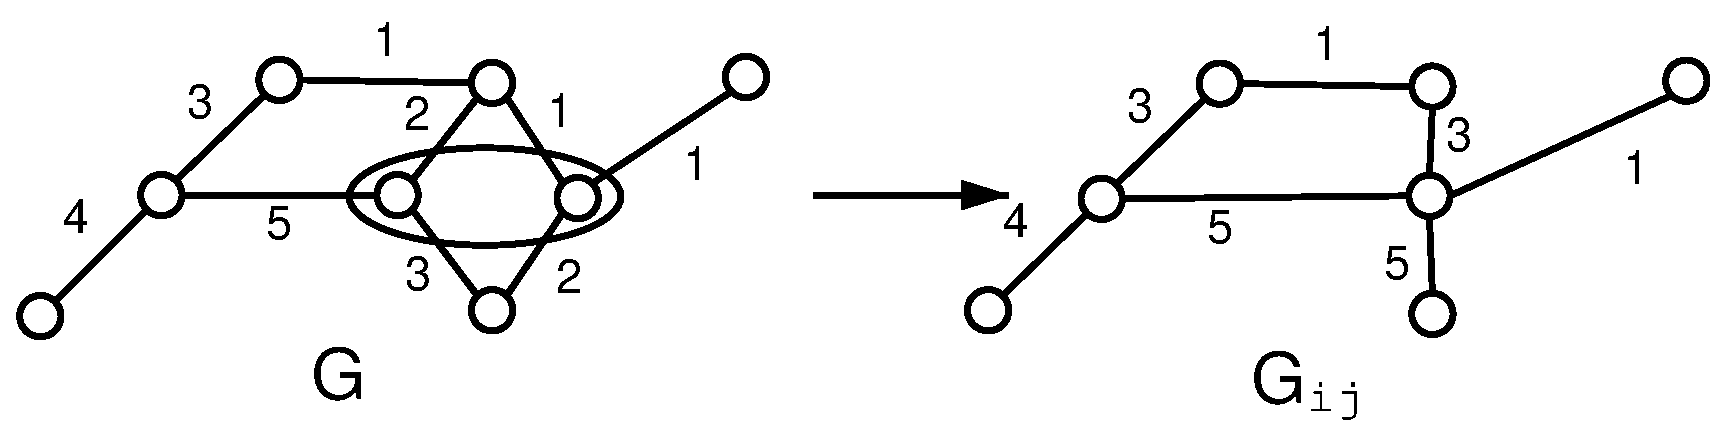
\includegraphics[height=3cm]{bilder/3-0KnotenSchrumpf}

$\lambda(G)$: Kapazität eines minimum Schnittes in $G$\\
$\lambda(G;i,j)$: Kapazität eines minimum i-j Schnittes in $G$

\begin{lemma}
$\lambda(G) = \min(\lambda(G_{i j}), \; \lambda(G;i,j))$
\end{lemma}

Beweis: trivial

\paragraph{Das Verfahren} \mbox{}\\
{
\renewcommand{\labelitemi}{\mbox{}}
\renewcommand{\labelitemii}{\mbox{}}
\renewcommand{\labelitemiii}{\mbox{}}
\renewcommand{\labelitemiv}{\mbox{}}
\begin{itemize}
\item $z^{\ast} := \infty$;
\item wiederhole $n-1$ mal:
\begin{itemize}
\item wähle $r,s \in V$;
\item Bestimme $(r,s)$-min-cut $\delta(S)$;
\item Falls $z(\delta(s)) < z^{\ast}$
\begin{itemize}
\item $S^{\ast} := S$;
\item $z^{\ast} := z(\delta(S))$;
\end{itemize}
\item Schrumpfe $r$ und $s$
\end{itemize}
\end{itemize}
}
liefert (mit G-T Algorithmus) eine Lösung in $O(n^{4})$ Zeit.

\subsubsection{Ein einfacher Min-Cut Algorithmus}

Grundidee: Nagamochi und Iberaki [1992]\\
Effiziente Implementierung von Nagamochi, Ono und Iberaki [1993]\\
einfache Korrektheitsbeweise: Frank [1994], Stoer u. Wagner [1994]\\
Beschreibung von Stoer und Wagner:\\
Notation $z(A:B)$: $\displaystyle \sum_{\begin{array}{c}a \in A\\b \in B
\end{array}} z_{ab} \; \; \mbox{ für } A, B \subseteq V$\\
$z(A:b)$ statt $z(A,\{b\})$

Erinnerung: Prims Algorithmus für einen minimum spannenden Baum: Min
Spanning Tree (G,z,a) [$a\in V$ beliebig].

\begin{algorithmic}
\STATE $W := \{a\}$;
\STATE $T := \varnothing$;
\WHILE{$W \not=V$}
\STATE wähle $v \not\in W$ mit $z_{w v} = \min \{z_{w v} | w \in W, w v \in
E\}$
\STATE $W := W \cup \{v\}$; \hspace{3mm} (Füge einen am schwächsten mit W
verbundenen Knoten hinzu)
\STATE $T := T \cup \{u v\}$;
\ENDWHILE
\end{algorithmic}
ähnlich:\\
{\bf Min\_Cut\_Phase}
\begin{algorithmic}
\STATE $W:= \{a\}$;
\WHILE{$W \neq V$}
\STATE wähle $v\not\in W $ mit $z(W:v) = \max\{z(W:v)|v \not\in W\}$;
\STATE $W:= W \cup \{v\}$; \hspace{3mm}(Füge einen am stärksten mit $W$ 
verb. Knoten hinzu)
\ENDWHILE
\STATE Sei $s$ der vorletzte, $t$ der vorletzte zu $W$ hinzugefügte Knoten.
\STATE $z^{\ast} := z(\delta(t))$;
\STATE $\delta^{\ast} :=$ Menge der von $t$ repräsentierten Orginalknoten
(Phasenschnitt);
\STATE Schrumpfe $s$ und $t$
\end{algorithmic}

{\bf Berechnung des Min-Cut($g,z,a$);}
\begin{algorithmic}
\STATE $z_{\min} := \infty$;
\WHILE{$|V| > 1$}
\STATE Min\_Cut\_Phase($G,z,a$);
\IF{$z^{\ast} < z_{\min}$}
\STATE $z_{\min} := z^{\ast}$;
\STATE $\delta_{\min} := \delta^{\ast}$;
\ENDIF
\ENDWHILE
\end{algorithmic}

\begin{lemma}
Jeder Phasenschnitt ist ein minimum $(s,t)$-Schnitt im jeweiligen
"`Phasengraphen"', wobei $s$ vorletzter und $t$ letzter zu $W$
hinzugefügter Knoten ist.
\end{lemma}

Beweis:\\
Situation: $\begin{array}{c}\stackrel{\mbox{\scriptsize
Hinzufügungsreihenfolge}}{\Longrightarrow}\\a \rightarrow \bullet \rightarrow 
\ldots \rightarrow s \rightarrow t\end{array}$\\
Sei $C \subseteq E$ ein beliebiger$(s,t)$-Schnitt in $G$\\
Wir zeigen $z(C) \geqq z^{\ast}=z(\delta(t))$\\
$v\neq a$ heißt {\it aktiv} bezüglich $C$, falls $w v \in C$ mit
$w=$ direkter Vorgänger von $v$.\\
$A_{v} \subseteq V$: Menge aller Vorgänger von $v$ (ohne $v$)\\
$C_{v} := \left\{x y \in C | x,y \in A_{v} \cup \{v\}\right\} \subseteq C$

Beispiel:

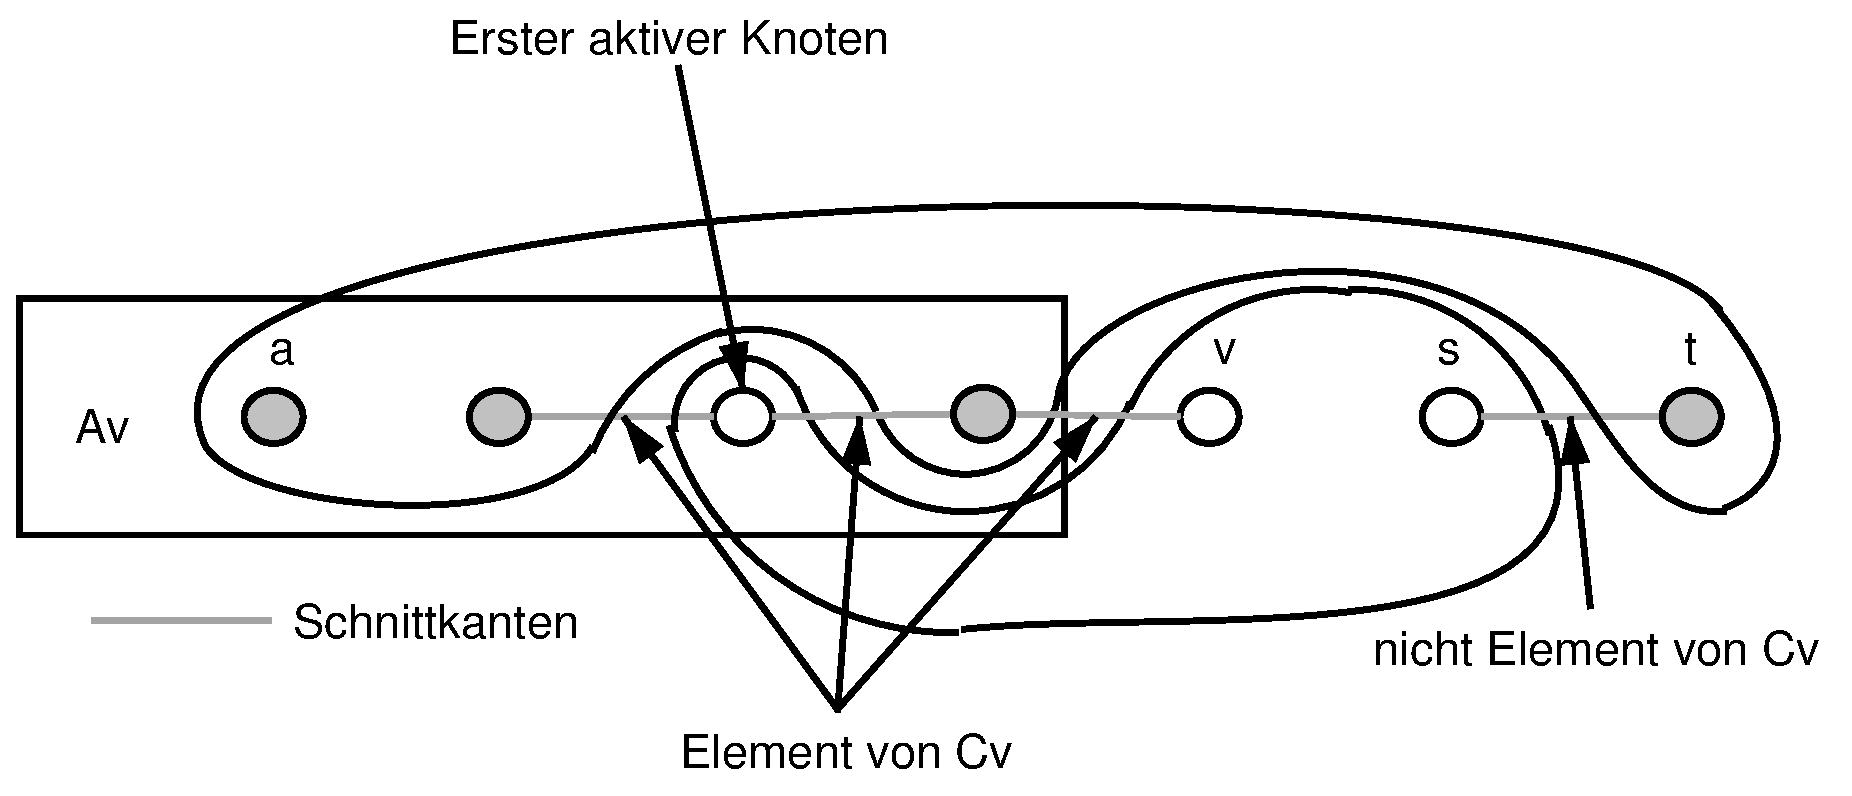
\includegraphics[width=12cm]{bilder/3-0Phasenschnitt1}

Behauptung: Für jeden aktiven Knoten gilt $z(A_{v}:v) \leqq z(C_{v})$.
Beweis: Induktion über aktive Knoten:\\
Für den ersten aktiven Knoten $v_{1}$ gilt $z(A_{v_{1}}:v_{1}) =
z(C_{v_{1}})$. Die Behauptung gelte für alle aktiven Knoten bis zu $v$. Sei
$n$ der nächste aktive Knoten.

Situation:\\
\[\underbrace{\underbrace{a \bullet\ldots \bullet}_{A_{v}\bullet}
\stackrel{\in C}{-} \underbrace{v\circ \ldots \circ}_{A_{u} \wout
A_{v}}}_{A_{u}}
\stackrel{\in C}{-}u \ldots s \ldots  t\]

Es gilt: $\begin{array}{rcl}z(A_{u}:u) &=& z(A_{v}:u) + z(A_{u} \wout A_{v} : 
u)\\
&\leqq& z(A_{v}:v) \hspace{5mm} (\mbox{Da $v$ stärkster mit $A_{v}$ verb.
Knoten})\\
&\leqq& z (C_{v})\\
&\leqq& z (C_{v}) + z ( A_{u} \wout A_{v} : u)
\end{array}$

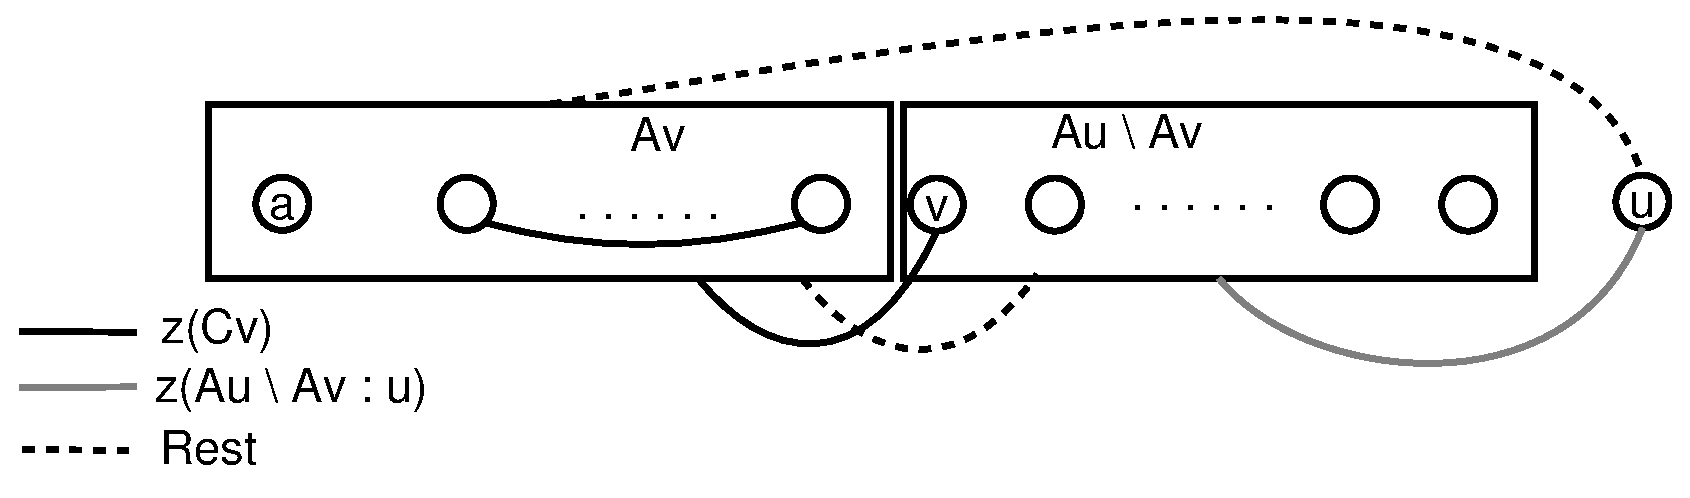
\includegraphics[width=12cm]{bilder/3-0Phasenschnitt2}

alles zusammen: $z(C_{u}) \leqq z(C_{u})$ q.e.d (Beh.)\\
$s t \in C \Rightarrow t \mbox{ aktiv } \Rightarrow  z^{\ast} = z(\delta(t))
= z(A_{t}:t) \leqq z(C_{t}) = z(C)$ q.e.d. (Lemma)

\paragraph{Laufzeit} \mbox{}\\
MINIMUM\_CUT\_PHASE\\
Prioritätsschlange für Knoten in $V\wout \{a\}$\\
\mbox{} \hspace{3mm}Schlüssel für $v \in V \wout \{a\}$\\
\mbox{} \hspace{6mm} key$(v) = z(W:v)$: Gesamtkapazität der Kanten zwischen
$v$ und derzeitigem $W$.
Neu hinzuzufügender Knoten $v$ via EXTRACT\_MAX\\
Update: key$(u) := key(u) + z_{v u}$ für $u \not \in W$ falls $v u \in E
\rightarrow$ INCREASE\_KEY\_OPERATION für jede Kante $e \in E$ genau einmal

insgesamt:\\
$\left. \begin{array}{rcll} n&=& |V| &\mbox{ EXTRACT\_MAX}\\
m&=& |E| &\mbox{ INCREASE\_KEY}\end{array} \right\}$ Operationen\\
mit Binär-Heaps (Informatik I) je:
$\left. \begin{array}{l} O(\log n)\\O(\log n)\end{array}\right\}$ Zeit\\
mit Fibonacci-Heaps je
$\left. \begin{array}{l}O(\log n)\\O(1)\end{array}\right\}$ Zeit

d.h. $O(m+n \log n)$ Zeit für MIN\_CUT\_PHASE\\
$O(n)$-Phasen $\rightarrow  O(m n + n^{2}\log n)$ Gesamtzeit.

\begin{satz}
Der Phasenschnitt-Algorithmus findet einen minimum Schnitt in einem
ungerichteten Graphen in $O(n m+n^{2}\log n)$ Zeit.
\end{satz}

In dieser Vorlesung teilte Prof. Jünger noch ein Blatt mit Beispielen zum
Phasenschnittalgorithmus sowie einen Artikel (Jünger M.; Rinaldi G.;
Thienel S. (2000). {\it Practical performance of efficient minimum cut
algorithms}. Algorithmica v26n1 S. 172-195).


